%AMRITA UNIVERSITY PH.D latex template...Created by Chungath, CYS-CBE%

\documentclass[a4paper, 12pt]{report}
%\renewcommand{\bibname}{References}
\usepackage[margin=0.8in]{geometry}
\usepackage{float}

\usepackage{bold-extra}
\usepackage{amsmath}
\usepackage{amsfonts}
\usepackage{amssymb}
\usepackage{graphicx}
\usepackage{xcolor}
\definecolor{silver}{HTML}{ECEEF1}
\usepackage [english]{babel}
\usepackage [autostyle, english = american]{csquotes}
\MakeOuterQuote{"}
%\usepackage[a4paper,top=30mm,bottom=30mm]{geometry}
\usepackage{setspace}
\onehalfspacing
\setlength{\emergencystretch}{3em}
\graphicspath{{images/}}
\usepackage{amsthm}
%\usepackage{hyperref}
%\hypersetup{colourlinks=true,linkcolour=blue}
\usepackage{array}
%\usepackage{parskip}
\usepackage{cite}
\usepackage{longtable}
\usepackage{fancyhdr}
\usepackage{titletoc}
\theoremstyle{definition}
\newtheorem{Definition}{Definition}[section]

%-------------------------------------------------------------
% title page
\begin{document}
	\pagenumbering{gobble}
	\thispagestyle{empty}
	\begin{large}
		\begin{center}
			{\Large\bfseries{DIGITAL TWIN ASSISTED DYNAMIC NETWORK SLICING USING SSL, TGNN AND MARL FOR AI-NATIVE 6G NETWORKS}}\\
			\vspace{1.3cm}
			A Thesis \\
			\vspace{.1cm}
			Submitted in partial fulfilment for the Degree of\\
			\vspace{.1cm}
			BACHELOR OF TECHNOLOGY\\
			\vspace{.1cm}
            in 
            \vspace{.1cm}
            \\ COMPUTER SCIENCE AND ENGINEERING (ARTIFICIAL INTELLIGENCE) \\
			\vspace{1cm}
			by\\ \vspace{0.2cm}
			\vspace{.1cm}
			{\Large\bfseries{Keerthivasan S V (CB.SC.U4AIE23037)}} \\ 
            {\Large\bfseries{Krish S (CB.SC.U4AIE23040)}} \\
            {\Large\bfseries{Sriranjana C (CB.SC.U4AIE23066)}} \\
            {\Large\bfseries{Thrishala S N (CB.SC.U4AIE23072)}} \\
            \vspace{3cm}
			
			
\includegraphics[scale=0.8]{univA.png}\\
			\vfill
			DEPARTMENT OF ARTIFICIAL INTELLIGENCE\\
			\Large{\textbf{AMRITA VISHWA VIDYAPEETHAM}}\\
			{\large COIMBATORE CAMPUS (INDIA)}\\
			\vspace*{.3cm}
			October 2026
		\end{center}
	\end{large}
	%------------------------------------------------------------------------------------
	% bonafide certificate
	\newpage
	\nopagecolor
	\begin{center}
		{\normalsize DEPARTMENT OF ARTIFICIAL INTELLIGENCE}\\
		{\large \textbf{AMRITA VISHWA VIDYAPEETHAM}}\\
		{\normalsize COIMBATORE CAMPUS}\\
		\vspace*{1.2cm}
		\includegraphics[width=0.42\textwidth]{univa.png}\\
		\vspace*{1.2cm}
		{\Large \textbf{BONAFIDE CERTIFICATE}}
	\end{center}
	\vspace*{.9cm}
	\noindent\begin{minipage}{\textwidth}
	\normalsize\setstretch{1.25}
	\noindent This is to certify that the thesis entitled \enquote{\textbf{Digital Twin Assisted Dynamic Network Slicing using SSL, TGNN and MARL for AI-Native 6G Networks}} submitted by \textbf{Keerthivasan S V (CB.SC.U4AIE23037)}, \textbf{Krish S (CB.SC.U4AIE23040)}, \textbf{Sriranjana C (CB.SC.U4AIE23066)}, and \textbf{Thrishala S N (CB.SC.U4AIE23072)} for the award of the \textbf{Degree of Bachelor of Technology} under the \textbf{Faculty of Engineering} is a bonafide record of the work carried out by them under my guidance and supervision in the Department of Artificial Intelligence, Amrita Vishwa Vidyapeetham, Coimbatore Campus.
	\end{minipage}
	\vspace*{3.5cm}

	\noindent Submitted for the examination held on \underline{\hspace{3.6cm}}.

	\vspace*{1cm}
	\noindent\textbf{INTERNAL EXAMINER}\hfill\textbf{EXTERNAL EXAMINER}
	\vspace*{3.2cm}

	\begin{center}
		\textbf{Dr. Sundaresan S}\\
		Thesis Advisor\\
		Department of Artificial Intelligence,\\
		Amrita Vishwa Vidyapeetham, Coimbatore Campus, India.
	\end{center}

	%-------------------------------------------------------------------------------
	% Declaration page
	\newpage
	\begin{center}
		{\normalsize DEPARTMENT OF ARTIFICIAL INTELLIGENCE}\\
		{\large \textbf{AMRITA VISHWA VIDYAPEETHAM}}\\
		{\normalsize COIMBATORE CAMPUS}\\
		\vspace*{1.2cm}
		\includegraphics[width=0.42\textwidth]{univa.png}\\
		\vspace*{1.2cm}
		{\Large \textbf{DECLARATION}}
	\end{center}
	\vspace*{.9cm}
	\noindent  We, \textbf{Keerthivasan S V., Roll. No: CB.SC.U4AIE23037}, \textbf{Krish S., Roll. No: CB.SC.U4AIE23040}, \textbf{Sriranjana C., Roll. No: CB.SC.U4AIE23066} and \textbf{Thrishala S N., Roll. No: CB.SC.U4AIE23072} hereby declare that this thesis entitled \enquote{\textbf{DIGITAL TWIN ASSISTED DYNAMIC NETWORK SLICING USING SSL, TGNN AND MARL FOR AI-NATIVE 6G NETWORKS}} is the record of the original work done by us under the guidance of \textbf{Dr. Sundaresan S}, Assistant Professor, Department of Artificial Intelligence, Amrita Vishwa Vidyapeetham, Coimbatore Campus. To the best of our knowledge, this work has not formed the basis for the award of any degree/diploma/associateship/fellowship or a similar award to any candidate in any University.\\\\
	
	\vspace*{1cm}
	\noindent{\bf Place:\hfill Signature of the Students} \\
	\noindent {\bf Date: }
	\vfill
	\begin{center}
		\large{COUNTERSIGNED}\\
	\end{center}
	\vspace{0.6in}
	
\begin{center}
		\textbf{Dr. K.P Soman}\\
	Professor and Dean, \\ 
	Department of Artificial Intelligence \\ Amrita Vishwa Vidyapeetham,\\
	Coimbatore Campus,\\
	India.
\end{center}
	
	%-----------------------------------------------------------------------------
	\clearpage
	\pagenumbering{roman}
	\tableofcontents
	
	\chapter*{Acknowledgements}
\addcontentsline{toc}{chapter}{Acknowledgements}
We express our sincere gratitude to our thesis advisor, Dr. Sundaresan S, for guidance and constructive feedback throughout this project. His questions about why a multi-agent controller is needed, and how a forecast should be shown to help, shaped the experiments in this thesis. We thank the faculty and review panel of the Department of Artificial Intelligence for helping us sharpen the problem statement and connect the implementation to a defensible evaluation.

\hspace{1.5em}We thank Amrita Vishwa Vidyapeetham, Coimbatore Campus, for the academic environment in which this work was undertaken, and Dr. K.P. Soman, Professor and Dean of the Department of Artificial Intelligence, for the facilities provided. We also acknowledge the creators of the public datasets and the maintainers of the open-source software on which this work builds: the Telecom Italia Big Data Challenge, 5G-NIDD, NeversNet5G and the B5G slicing dataset, and OMNeT++, INET, Simu5G, PyTorch and PyTorch Geometric. Their openly available data and documentation made it possible to concentrate on the unified environment, fair evaluation and the Digital Twin.

\hspace{1.5em}We thank our teammates, friends and families for their support. The responsibility for the implementation choices, the interpretation of results and the remaining limitations rests with the authors.

\vspace{1cm}
\begin{flushright}
KEERTHIVASAN S V\\
KRISH S\\
SRIRANJANA C\\
THRISHALA S N
\end{flushright}
\clearpage
\listoffigures
	\addcontentsline{toc}{chapter}{List of figures}
	\listoftables
	\addcontentsline{toc}{chapter}{List of tables}
	\newpage
%\chapter*{Abbreviations}

% Abbreviations and List of Symbols for the thesis
% Paste these sections where the corresponding sections appear in the main file.
% Required packages already present in the thesis preamble: longtable, array, amsmath.

% -------------------- Abbreviations --------------------
\section*{{\huge Abbreviations}\hfill}
\addcontentsline{toc}{chapter}{\textbf{Abbreviations}}
\vspace{0.5cm}

\begin{longtable}{p{3.2cm} p{11cm}}
6G & Sixth-generation mobile communication network \\
AI & Artificial intelligence \\
DDPG & Deep deterministic policy gradient \\
DL & Downlink \\
DT & Digital Twin \\
eMBB & Enhanced mobile broadband \\
GNN & Graph neural network \\
gNB & Next-generation Node B; a 5G/6G base station \\
GAE & Generalised advantage estimation \\
GRU & Gated recurrent unit \\
IPPO & Independent proximal policy optimisation \\
LLM & Large language model \\
MAE & Mean absolute error \\
MADDPG & Multi-agent deep deterministic policy gradient \\
MAPE & Mean absolute percentage error \\
MAPPO & Multi-agent proximal policy optimisation \\
MARL & Multi-agent reinforcement learning \\
MCP & Model Context Protocol \\
MLP & Multilayer perceptron \\
mMTC & Massive machine-type communication \\
MSE & Mean squared error \\
NDT & Network Digital Twin \\
NR & New Radio \\
O-RAN & Open Radio Access Network \\
PPO & Proximal policy optimisation \\
POMDP & Partially observable Markov decision process \\
PRB & Physical resource block \\
QoS & Quality of service \\
RAN & Radio access network \\
RL & Reinforcement learning \\
RMSE & Root mean squared error \\
SCARF & Self-supervised contrastive learning using random feature corruption \\
SLA & Service level agreement \\
SINR & Signal-to-interference-plus-noise ratio \\
SSL & Self-supervised learning \\
TGNN & Temporal graph neural network \\
UE & User equipment \\
URLLC & Ultra-reliable low-latency communication \\
VNF & Virtual network function \\
\end{longtable}

\newpage

% -------------------- List of Symbols --------------------
\section*{{\huge List of Symbols}\hfill}
\addcontentsline{toc}{chapter}{\textbf{List of Symbols}}
\vspace{0.5cm}

\begin{longtable}{p{3.2cm} p{11cm}}
$i$ & Index of a network cell or cell-level agent \\
$t$ & Time-step or traffic interval index \\
$\mathcal{V}$ & Set of cells (nodes) in the network graph \\
$\mathcal{E}$ & Set of edges representing connections or neighbourhood relations between cells \\
$\mathcal{G}=(\mathcal{V},\mathcal{E})$ & Network graph, consisting of cells and their relationships \\
$s_t^i$ & State or observation available to the agent controlling cell $i$ at time $t$ \\
$a_t^i$ & Allocation action selected by the agent for cell $i$ at time $t$ \\
$R_t^i$ & Reward received by the agent controlling cell $i$ at time $t$ \\
$S_t^i$ & Weighted service-level-agreement (SLA) score for cell $i$ at time $t$ \\
$F_t^i$ & Fraction of demand served by cell $i$ at time $t$ \\
$H_t^i$ & Reconfiguration churn for cell $i$ at time $t$ \\
$D_{t,k}^i$ & Demand for slice $k$ in cell $i$ at time $t$ \\
$\widehat{D}_{t+1,k}^i$ & Forecast demand for slice $k$ in cell $i$ for the next interval \\
$C_t^i$ & Usable capacity of cell $i$ at time $t$ \\
$x_{t,k}^i$ & Fraction of cell $i$'s capacity allocated to slice $k$ at time $t$ \\
$x_{t,\mathrm{idle}}^i$ & Fraction of cell $i$'s capacity left idle at time $t$ \\
$k$ & Index identifying a network slice, such as eMBB, URLLC or mMTC \\
$L$ & Network latency or packet/frame delay, depending on the reported experiment \\
$J$ & Jitter, representing variation in packet/frame delay \\
$\rho$ & Reliability or probability of successful service, when used in the SLA definition \\
$\mathbf{z}_t^i$ & Learned feature representation (embedding) for cell $i$ at time $t$ \\
$\widehat{\mathbf{y}}_t$ & Model-predicted value or traffic demand; the exact target depends on the experiment \\
\end{longtable}

% Notes:
% 1. The reward equation in Chapter 4 defines
%    R_t^i = 0.7 S_t^i + 0.3 F_t^i - 0.1 H_t^i.
% 2. Keep only symbols that are used in the final thesis text/equations.
% 3. If the thesis uses a different notation for any quantity, update the entry here
%    to match the notation used in the relevant chapter.
	

\newpage

\chapter*{Abstract}
\addcontentsline{toc}{chapter}{Abstract}
Network slicing lets enhanced mobile broadband (eMBB), ultra-reliable low-latency communication (URLLC) and massive machine-type communication (mMTC) services share one infrastructure. Most slicing controllers only react once demand has already changed. In this thesis we ask two questions: does it help to predict traffic before bandwidth is allocated, and is a decentralised multi-agent controller a better design than one central controller?

We built a pipeline of self-supervised learning (SSL), a temporal graph neural network (TGNN) forecaster and multi-agent reinforcement learning (MARL), and tested it in a Digital Twin. No public dataset combines topology, per-slice traffic, quality of service and allocation actions, so we made a unified slicing environment from real Telecom Italia Milan traffic (62 days, 10{,}000 cells), with latency calibrated on a public 6G RAN telemetry dataset. All results are measured on a held-out week, and the controllers were chosen on separate validation days.

A MARL controller with shared parameters keeps one actor of 19{,}332 parameters from 9 to 100 cells. A single central agent grows to 604{,}048 parameters and its reward falls from about 0.43 to 0.27. We also compared with rule-based controllers whose targets were tuned on the training days. With a long training budget and averaged seeds, the off-policy learned controller beats them on all seven test days at every size we tried, by 0.023 to 0.026 in reward. It only matches a richer rule that is tuned for each time of day and cell class. An on-policy (PPO-family) learner does beat that rule on every test day, by 0.009 in reward at 25 cells.

A TGNN trained on 39 days beats persistence on all 10{,}000 cells (its mean squared error is lower by 18\%, 33\% and 31\% for eMBB, URLLC and mMTC). Giving its forecast to the rule-based controller raises the reward by about 0.03, which closes about one fifth of the gap to perfect knowledge of the next interval. We have not shown that the forecast helps the learned controller. Self-supervised pretraining, tested on de-duplicated data with different numbers of labels, gave no gain over strong raw-feature baselines, and we report this as a negative result.

The Digital Twin works as an approval gate that protects the reward from poor proposals. A packet-level Simu5G sweep agrees with our calibrated QoS model on the order of delays but not on the shape of the delay curve. We also release a Digital Twin dataset of 393.6 million rows with six what-if scenarios, and an interactive monitor, Slice Twin, which is published on the web.

\vspace{0.4cm}
\noindent \textbf{Keywords:} network slicing, 6G, Digital Twin, self-supervised learning, temporal graph neural network, multi-agent reinforcement learning, traffic forecasting.

\clearpage
\pagenumbering{arabic}
\setcounter{page}{1}
\chapter{Introduction}
\label{chap.1}
\section{Background and Motivation}
Sixth-generation networks will have to carry very different services over the same radios. Streaming video and extended reality want high throughput (enhanced mobile broadband, eMBB). Factory control and connected vehicles want a delay of a few milliseconds and almost no loss (ultra-reliable low-latency communication, URLLC). Sensor networks want to connect huge numbers of cheap devices that each send very little (massive machine-type communication, mMTC).

Network slicing is the usual answer. The operator cuts the radio and core resources into logical slices and promises each slice a service level agreement (SLA). The difficult part is deciding how big each slice should be, because demand keeps moving and is different in every cell. A fixed split wastes capacity when a slice is quiet and breaks the SLA when it is busy. Learning-based controllers do better, but most of the ones we found in the literature only look at what the network is doing right now, so they react after the demand has already moved.

\section{Problem Statement}
We ask two questions in this thesis.
\begin{enumerate}
	\item Can a slicing controller that is told the demand of the next interval allocate bandwidth better than one that sees only the current demand?
	\item Is a decentralised multi-agent controller a better solution to this task than a single central agent?
\end{enumerate}
We also want to try such controllers in a Digital Twin (DT) before anyone would use them on a real network.

\section{Proposed Approach}
Our pipeline has four stages (Table~\ref{tab:pipeline}). A self-supervised learning (SSL) encoder is trained on unlabelled telemetry and gives a compact description of each observation. A temporal graph neural network (TGNN) predicts the demand of every slice in the next interval; it mixes information from neighbouring cells with GraphSAGE \cite{hamilton2017} and follows each cell through time with a recurrent update. A multi-agent reinforcement learning (MARL) controller, with one agent per cell, then splits the capacity of its cell between eMBB, URLLC, mMTC and an idle share. The Digital Twin is a virtual copy of the network where these allocations are trained, tested and, if possible, approved before they are applied.

\begin{table}[h]
	\centering
	\caption{Stages of the proposed pipeline}
	\label{tab:pipeline}
	\begin{tabular}{|p{2.8cm}|p{6.5cm}|p{4.2cm}|}
		\hline
		\textbf{Stage} & \textbf{Role} & \textbf{Output} \\ \hline
		Self-supervised learning & Learns representations of telemetry from unlabelled data by masking or corrupting features and recovering them & Embedding per node and time step \\ \hline
		Temporal GNN & Forecasts next-interval demand per cell and slice from the cell graph and recent history & Predicted demand \\ \hline
		Multi-agent RL & Each cell agent decides how to split its bandwidth between slices & Slice shares per cell \\ \hline
		Digital Twin & Virtual network that trains, tests and checks allocations and supports what-if scenarios & Evaluation, approval, scenario data \\ \hline
	\end{tabular}
\end{table}

\section{Objectives and Contributions}
\subsection{Objectives}
\begin{enumerate}
	\item Survey the literature on Digital Twins, SSL, graph-based forecasting and MARL for network slicing and identify the research gap.
	\item Collect and prepare public data for each stage of the pipeline.
	\item Implement each module and evaluate it against strong, simple baselines on real data.
	\item Provide one environment in which prediction and allocation are tested together on the same traffic.
	\item Build a working prototype.
\end{enumerate}

\subsection{Contributions}
Each contribution below is supported by experiments in the later chapters, and the limits of each are stated there.
\begin{enumerate}
	\item \textbf{A unified slicing environment.} No public dataset combines topology, per-slice traffic, quality of service (QoS) and allocation actions. We built one from real Telecom Italia Milan traffic, with latency calibrated on a public 6G radio access network (RAN) telemetry dataset, and we mark every component as real, calibrated or modelled.
	\item \textbf{A fair evaluation of MARL.} A parameter-shared controller keeps a fixed-size actor from 9 to 100 cells while a central agent does not scale. Against expert rules tuned on the training days, it wins on all seven test days at every size (by 0.023 to 0.026 in reward), and an on-policy PPO-family learner also beats a rule tuned per time of day and cell class (by 0.009 at 25 cells, on every test day), whereas the off-policy learner only matches that rule.
	\item \textbf{A measurement of what prediction is worth.} Giving the expert rule the TGNN forecast raises its reward by about 0.03 on every test day, about one fifth of the gap to perfect knowledge. The benefit to the learned controller is not established.
	\item \textbf{A city-scale forecasting finding.} A forecaster trained only on the dense centre was 10.8 times worse than persistence in the outer city. Per-cell scaling, random spatial patches and more training days fixed this, and the retrained forecaster beats persistence in all 10{,}000 cells (18\%, 33\% and 31\% lower error for the three slices).
	\item \textbf{A clean negative result for SSL.} After removing duplicate flows and leaked columns, pretraining gave no gain over strong raw-feature baselines at any label budget, on 5G-NIDD and on the Milan forecaster.
	\item \textbf{A Digital Twin that checks decisions.} An approval gate in the environment protects the reward from poor proposals, and a Simu5G load sweep tests the QoS model against a packet-level simulator.
	\item \textbf{A dataset and a prototype.} A 393.6-million-row, 122-column dataset with six what-if scenarios, and the Slice Twin monitor, which is published on the web.
\end{enumerate}

\subsection{Scope}
The thesis does not cover the following.
\begin{itemize}
	\item A packet-level simulator inside the training loop. The QoS comes from a calibrated surrogate, and the telemetry used to calibrate it is itself simulated. Our own 19-gNodeB scenario is not connected to Simu5G; we only ran a single-cell load sweep.
	\item A statistically wide evaluation. Results use one held-out week (seven days), at most three seeds per learned controller (one at 100 cells), and one city.
	\item Deployment on a live or emulated network. The prototype replays recorded days.
\end{itemize}

\subsection{Organisation}
Chapter~\ref{chap.2} reviews the literature and the research gap, and Chapter~\ref{chap.3} describes the datasets and how we prepared them. Chapter~\ref{chap.4} presents the system design, the problem formulation and the unified environment. Chapters~\ref{chap.5}, \ref{chap.6} and \ref{chap.7} cover self-supervised representation learning, temporal GNN forecasting and MARL for slice allocation. Chapter~\ref{chap.8} gives the integrated evaluation, the Digital Twin dataset, the approval gate and the Simu5G check. Chapter~\ref{chap.9} describes the Slice Twin prototype, and Chapter~\ref{chap.10} ends with the limitations and future work.

\chapter{Literature Review and Research Gap}
\label{chap.2}

\section{Scope of the Review}
This chapter summarizes the literature on Digital Twins, self-supervised learning (SSL), graph-based forecasting, and reinforcement learning (RL) for slicing that is relevant to the four proposed building blocks of the pipeline. The papers studied span the years 2020–2026 from IEEE venues and some were arXiv or TechRxiv preprints. We picked up the method, data or simulator, results and research gap for each. The papers are summarized pillar wise in Table~\ref{tab:lit}.

\section{Digital Twins for Network Slicing}
In \cite{nativendt2025} a three-layer native Network Digital Twin (NDT) architecture, with a four-stage lifecycle (preparation, creation, runtime, feedback) was proposed. In an operator-inspired signalling-storm scenario, it achieved approximately 3\% MAPE when considering the registration arrival rate and approximately 25\% for the successful registration count, but it only allows for simulation and verification and does not include any GNN, SSL or RL. Graph-based twins predict network KPIs: one predicts end-to-end slice latency with less than 5\% error on NSFNET, GEANT2 and a synthetic topology with 50 nodes \cite{gnndt2022}; a virtualisation-aware twin adds graph attention to improve performance over RouteNet-Fermi \cite{attentionvirt2025}; a decentralised GNN twin addresses end-to-end slicing \cite{dte2e2023}. These twins are based on the static graphs and supervised learning. Twins with control agents are still reactive: using a clean telemetry in the same way, a twin-synchronised DDPG agent reduced latency by approximately 25\% compared to static allocation \cite{ali2025}; an NDT agent on the Milan data (of about 10,000 cells) achieved 25.5\% less load and 30.4\% less energy savings with a rolling-average predictor \cite{selfopt2026}.

\section{Self-Supervised Learning for Wireless Data}
A survey on SSL for wireless networks is presented that investigates the generative and contrastive and predictive paradigm and the integration with Digital Twins, TGNNs and reinforcement learning is still not widely explored \cite{sslwireless2024}. Net2Net learns node embeddings from predicting the position and achieves better results than baselines on eight graph datasets, with only static and non-telecom graphs \cite{net2net2025}. For network traffic, two-stage SSL was able to achieve 97.64\% accuracy on network traffic classification for encrypted traffic in SDN, which is approximately 2\% higher than a supervised model \cite{sslsdn2022}; autoencoder with tabular contrastive learning and Confident Learning achieved improved label noise reduction on three traffic datasets \cite{sslcl2025}. The use of SSL is therefore one of classification or non-telecom graphs, and is uncommon for slicing telemetry.

\section{Traffic Forecasting for Slicing}
The Holt-Winters forecasting has been integrated with adaptive VNF scaling for slicing, however, only in simulated topology and traffic \cite{holtwinters2020} and DeepCog forecasts capacity for slice provisioning \cite{bega2020deepcog}. Compared to other graph-based methods, SSGNN achieves best improvements of up to 3.0\% in MAE, 5.2\% in RMSE and 3.8\% in MAPE across six road-traffic datasets \cite{ssgnn2023}. It forecasts road traffic and the forecast is not linked to any allocation decision.

\section{Reinforcement Learning for Slicing}
Other representative multi-agent approaches to slicing include SF-DTMC with an adaptive retention framework that reduced reconfiguration time and SLA violations in NS-3 but was limited to local cell clusters and reactive observations \cite{li2026}; MADDPG for vehicular slicing, achieving 96.5\% QoS satisfaction with coordination delays ranging from 120--180 ms which violate URLLC budgets \cite{vehicularmarl2023}; and an improved MADDPG with rank voting for multi-objective allocation, with no Pareto guarantee \cite{imaddpg2023}. Other work include: GAN-DDPG with a semantic-aware reward (22\% and 20\% higher URLLC and eMBB spectral efficiency, respectively, and 31\% lower packet loss) \cite{john2026} ; DRL for end-to-end slicing on a real testbed (where safety DRL cut SLA violations from up to 15\% to about 1\%, and learning on a real network is slow and potentially unsafe) \cite{drle2e2023} ; slice mobility by optimisation and game theory \cite{slicemobility2022} ; online learning for AI-service slicing \cite{slicingforai2025} ; an agentic LLM control plane with closed-loop SLA monitoring \cite{agentic2026} ; and a conceptual semantic ``Reasoning Plane'' \cite{chowdhury2025}. This thesis aims to place the semantic slicing framework as future work.


{\footnotesize\setstretch{1}
\begin{longtable}{|p{0.9cm}|>{\raggedright\arraybackslash}p{4.8cm}|>{\raggedright\arraybackslash}p{4.7cm}|>{\raggedright\arraybackslash}p{4.5cm}|}
\caption{Summary of the reviewed papers by pillar}\label{tab:lit}\\
\hline
\textbf{Ref.} & \textbf{Method} & \textbf{Data used} & \textbf{Gap} \\ \hline
\endfirsthead
\hline
\textbf{Ref.} & \textbf{Method} & \textbf{Data used} & \textbf{Gap} \\ \hline
\endhead
\multicolumn{4}{|l|}{\textit{Digital Twin}} \\ \hline
\cite{nativendt2025} & Three-layer native NDT, gray-box modelling & Signalling-storm scenario (private) & Single use case; no GNN, SSL or RL \\ \hline
\cite{gnndt2022} & GraphSAGE twin for end-to-end latency & NSFNET, GEANT2, synthetic & Static graph; supervised \\ \hline
\cite{attentionvirt2025} & GraphSAGE + graph attention, virtualisation-aware & Docker UPF, extended OMNeT++ & Static graph; supervised \\ \hline
\cite{dte2e2023} & Decentralised GNN twin & OMNeT++ (120,000 train, 3,120 validation) & Real-time data, diverse traffic, isolation, SLA unresolved \\ \hline
\cite{ali2025} & Twin synchronisation + DDPG & Own Python 5G simulator & Clean telemetry assumed; reactive \\ \hline
\cite{selfopt2026} & Rolling average, Isolation Forest, MLP & Milan (public) & Simple predictor; one dataset \\ \hline
\multicolumn{4}{|l|}{\textit{Self-supervised learning}} \\ \hline
\cite{sslwireless2024} & Survey of SSL paradigms & None (survey) & Integration with twins, TGNN, RL unexplored \\ \hline
\cite{net2net2025} & Position-prediction SSL & Eight non-telecom graph datasets & Static graphs \\ \hline
\cite{sslsdn2022} & Pre-training and fine-tuning & Mininet, D-ITG traffic & Classification only \\ \hline
\cite{sslcl2025} & Autoencoder, contrastive learning, Confident Learning & ISCX VPN-nonVPN, UCDavis--QUIC, own flows & Limited datasets; generalisation unvalidated \\ \hline
\multicolumn{4}{|l|}{\textit{Forecasting}} \\ \hline
\cite{holtwinters2020} & Holt-Winters, VNF scaling, DPSO and annealing placement & Simulated 5G topology and traffic & No real-world validation; scalability \\ \hline
\cite{ssgnn2023} & Masked SSL, spatio-temporal GNN, self-distillation & METR-LA, PEMS-BAY, PEMS03/04/07/08 & Road traffic; not used for allocation \\ \hline
\multicolumn{4}{|l|}{\textit{Reinforcement learning and slicing management}} \\ \hline
\cite{li2026} & SF-DTMC in RAN-POSG & NS-3 simulator & Local clusters; reactive \\ \hline
\cite{vehicularmarl2023} & POMDP, MADDPG & Mininet, Ryu & Simulation only; delays exceed URLLC budget \\ \hline
\cite{imaddpg2023} & MADDPG with rank voting & Simulated RAN, three slice types & Simulation; no Pareto guarantee \\ \hline
\cite{john2026} & GAN-DDPG, semantic reward & Custom 6G simulator & Domain-specific semantic states \\ \hline
\cite{drle2e2023} & Safety, distributed and imitation DRL & OpenAirInterface/FlexRAN testbed & Reactive; real-network learning unsafe \\ \hline
\cite{slicemobility2022} & Optimisation, game theory & Discrete-time simulation & Optimisation-based; no SSL, TGNN or MARL \\ \hline
\cite{slicingforai2025} & Online learning (EXP3) & Mobile-health dataset & No forecasting, no MARL \\ \hline
\cite{agentic2026} & LLM agents, MCP, SLA monitoring & Slice-specification, manifest and intent data; Open5GS and Ericsson RAN testbed & Large-scale, multi-domain, adversarial robustness \\ \hline
\cite{chowdhury2025} & Semantic Reasoning Plane & None (conceptual) & Added latency not quantified \\ \hline
\end{longtable}
}


\section{Data Used in the Reviewed Work}
The remaining twelve papers rely on data from a simulator, emulator or testbed, while only one paper relies on public cellular traffic, which is also used by us \cite{selfopt2026}. None use a public data set that includes topology, per-slice traffic, QoS and allocation decisions, so generating that data is the common practice, which is accommodated by the unified environment of Chapter~
ef{chap.4}.

\section{Research Gap}
Individual components of our pipeline are discussed in the literature: reinforcement learning-based twins, slicing using MARL, and forecasting using GNN. Most controllers use the current state; forecasts are seldom related to allocations; graph models are based on static graphs or road traffic; and multi-agent work is tested on small clusters and own simulators. We did not identify a paper that integrates the combination of SSL, temporal graph forecasting, a Digital Twin and MARL for slicing, while other papers we reviewed included an overview of the different building blocks but not how the forecasts are used to allocate. This thesis is a test of forecasting and multi-agent allocation jointly on real city-scale traffic.
\chapter{Datasets and Data Preparation}
\label{chap.3}
\section{Introduction}
Different kinds of data are required at each stage of the pipeline and no one source contains all of these. This chapter outlines the datasets gathered for the project, the reasons that none of these constitute a single dataset and the limitations associated with each. Table~\ref{tab:datasets} lists the datasets that were collected and used.

\section{Datasets Used}
Table~\ref{tab:datasets} gives the size, contents, role and preprocessing of each dataset.

{\footnotesize
\begin{longtable}{|p{2.3cm}|p{2.5cm}|p{3.3cm}|p{2.6cm}|p{2.6cm}|}
\caption{Datasets used in the project}
\label{tab:datasets}\\
\hline
\textbf{Dataset} & \textbf{Size} & \textbf{Contents} & \textbf{Role} & \textbf{Preprocessing} \\ \hline
\endfirsthead
\hline
\textbf{Dataset} & \textbf{Size} & \textbf{Contents} & \textbf{Role} & \textbf{Preprocessing} \\ \hline
\endhead
Telecom Italia Milan & 62 days, 10,000 cells, 10-minute intervals & SMS, call and internet activity on a $100 \times 100$ grid of 235\,m cells & Real traffic for SSL, TGNN, the unified environment and the Digital Twin dataset & Internet, calls and SMS mapped to eMBB, URLLC and mMTC demand; per-cell 95th-percentile scaling for the city-wide forecaster \\ \hline
5G-NIDD & 1{,}215{,}890 flows (408{,}655 unique) & Labelled benign and attack flows from a 5G network & Training and evaluation of the SSL encoder & Exact duplicates and identifier columns removed{,} log scaling{,} one-hot encoding{,} stratified 80/20 split \\ \hline
NeversNet5G & 716 UE files, about 27\,GB, 19 gNodeBs & Vehicular 5G NR telemetry produced with Simu5G and SUMO & UE to gNodeB topology (695 nodes) and telemetry replay & Graph built by nearest-gNodeB association \\ \hline
B5G network slicing & 7,984 samples & Transport topologies with eMBB, URLLC and mMTC flows & First MARL environment & Train, validation and test split \\ \hline
6G RAN telemetry & 30,000 windows & PRB load, latency percentiles, SLA flag and reward & Calibration of latency against load & Latency and jitter curves fitted against load \\ \hline
DeepSlice, Secure5G, Kaggle slicing sets, Botez 6G slicing & Small & Slice labels and QoS budgets & Slice-type benchmarks & --- \\ \hline
\end{longtable}
}

\section{Is there a Unified Public Dataset?}
A dataset that links all the stages of the pipeline would have to hold, in one record, the topology of the network, the traffic of each cell over time, the demand of each slice, QoS measurements, the SLA outcome, and the allocation action taken with its reward. We searched the datasets we hold and the web, and none of them contains all of these.

The closest is the B5G slicing dataset, which covers only the transport network and has no record of allocation actions. Published O-RAN slicing traces come from single-cell testbeds, and we could not confirm that they are released. The literature audit of Chapter~\ref{chap.2} agrees: of the sixteen papers reviewed, eight use their own data sets, and none releases a public dataset with topology, per-slice traffic, QoS and allocation decisions together.

On the advice of our guide we therefore built a unified dataset synthetically, based on real data wherever real data exist. The environment is described in Chapter~\ref{chap.4} and the data it generates in Chapter~\ref{chap.8}.

\section{Dataset Limitations}
Each source limits what the experiments can show.
\begin{itemize}
	\item \textbf{Telecom Italia Milan} has no network-control information: no PRB allocation, slice configuration, latency, QoS or SLA decisions, and no MARL actions. It supplies the real traffic-demand layer only, and the demand of each slice is assumed from it.
	\item \textbf{B5G} models the transport network and not the RAN. The samples used do not include latency or loss, so the reward of the first MARL environment is nearly trivial, and no Digital Twin loop could approve actions on it.
	\item \textbf{6G RAN telemetry} calibrates latency against load, but the telemetry is itself simulated. The calibration therefore ties the environment to a model and not to measurements from an operating network.
	\item \textbf{NeversNet5G} was produced with Simu5G and SUMO and not on a real deployment.
	\item \textbf{5G-NIDD} is a labelled intrusion-detection dataset. It can evaluate the SSL encoder, but it holds no slicing information. About two thirds of its flows are exact duplicates (807{,}235 of 1{,}215{,}890), which would leak between a random training and test split, so only the unique flows are used.
\end{itemize}

\chapter{System Design and the Unified Slicing Environment}
\label{chap.4}

\section{Overview}
The four phases of the proposed pipeline (Table~\ref{tab:pipeline}) can only be evaluated collectively, if the forecast, allocation and the resulting service quality are known for the same cell within the same interval. This chapter outlines this: the formulation of the slicing task, unified environment for evaluation of forecast and allocations in the testbed, calibration process for the testbed's quality-of-service (QoS) model, and reference policies used to compare learned controllers.

A dataset that links these phases would have to hold, in one record, the network topology, the traffic of each cell over time, the demand of each slice, QoS measures, the SLA outcome, and the allocation action with its reward. We reviewed the datasets we hold and searched for others, and none has all of these. The closest are the B5G slicing dataset, which covers only the transport network and has no allocation actions, and published O-RAN slicing traces, which come from single-cell testbeds and whose release we could not verify. We therefore built the unified environment synthetically, based on real data wherever real data exist.

\section{System Architecture}
The architecture of the proposed system consists of eight stages, as shown in Figure~\ref{fig:arch}. Network data are gathered from multiple sources (stage 1). Self-supervised learning learns representations from unlabelled network data (stage 2), while the temporal graph neural network makes predictions for future traffic and network states using temporal graphs (stage 3). Multiple MARL agents make joint decisions (stage 4). These decisions are executed in the Digital Twin, which is a virtual copy of the network (stage 5), and resources are assigned to the network slices according to the predictions (stage 6). The network state in the Digital Twin is updated (stage 7), and its performance is evaluated to calculate the reward to improve the policies of the agents (stage 8). Stages 5 to 8 are implemented in the unified environment presented in Section~\ref{sec:env}.
 
\begin{figure}[h]
\centering
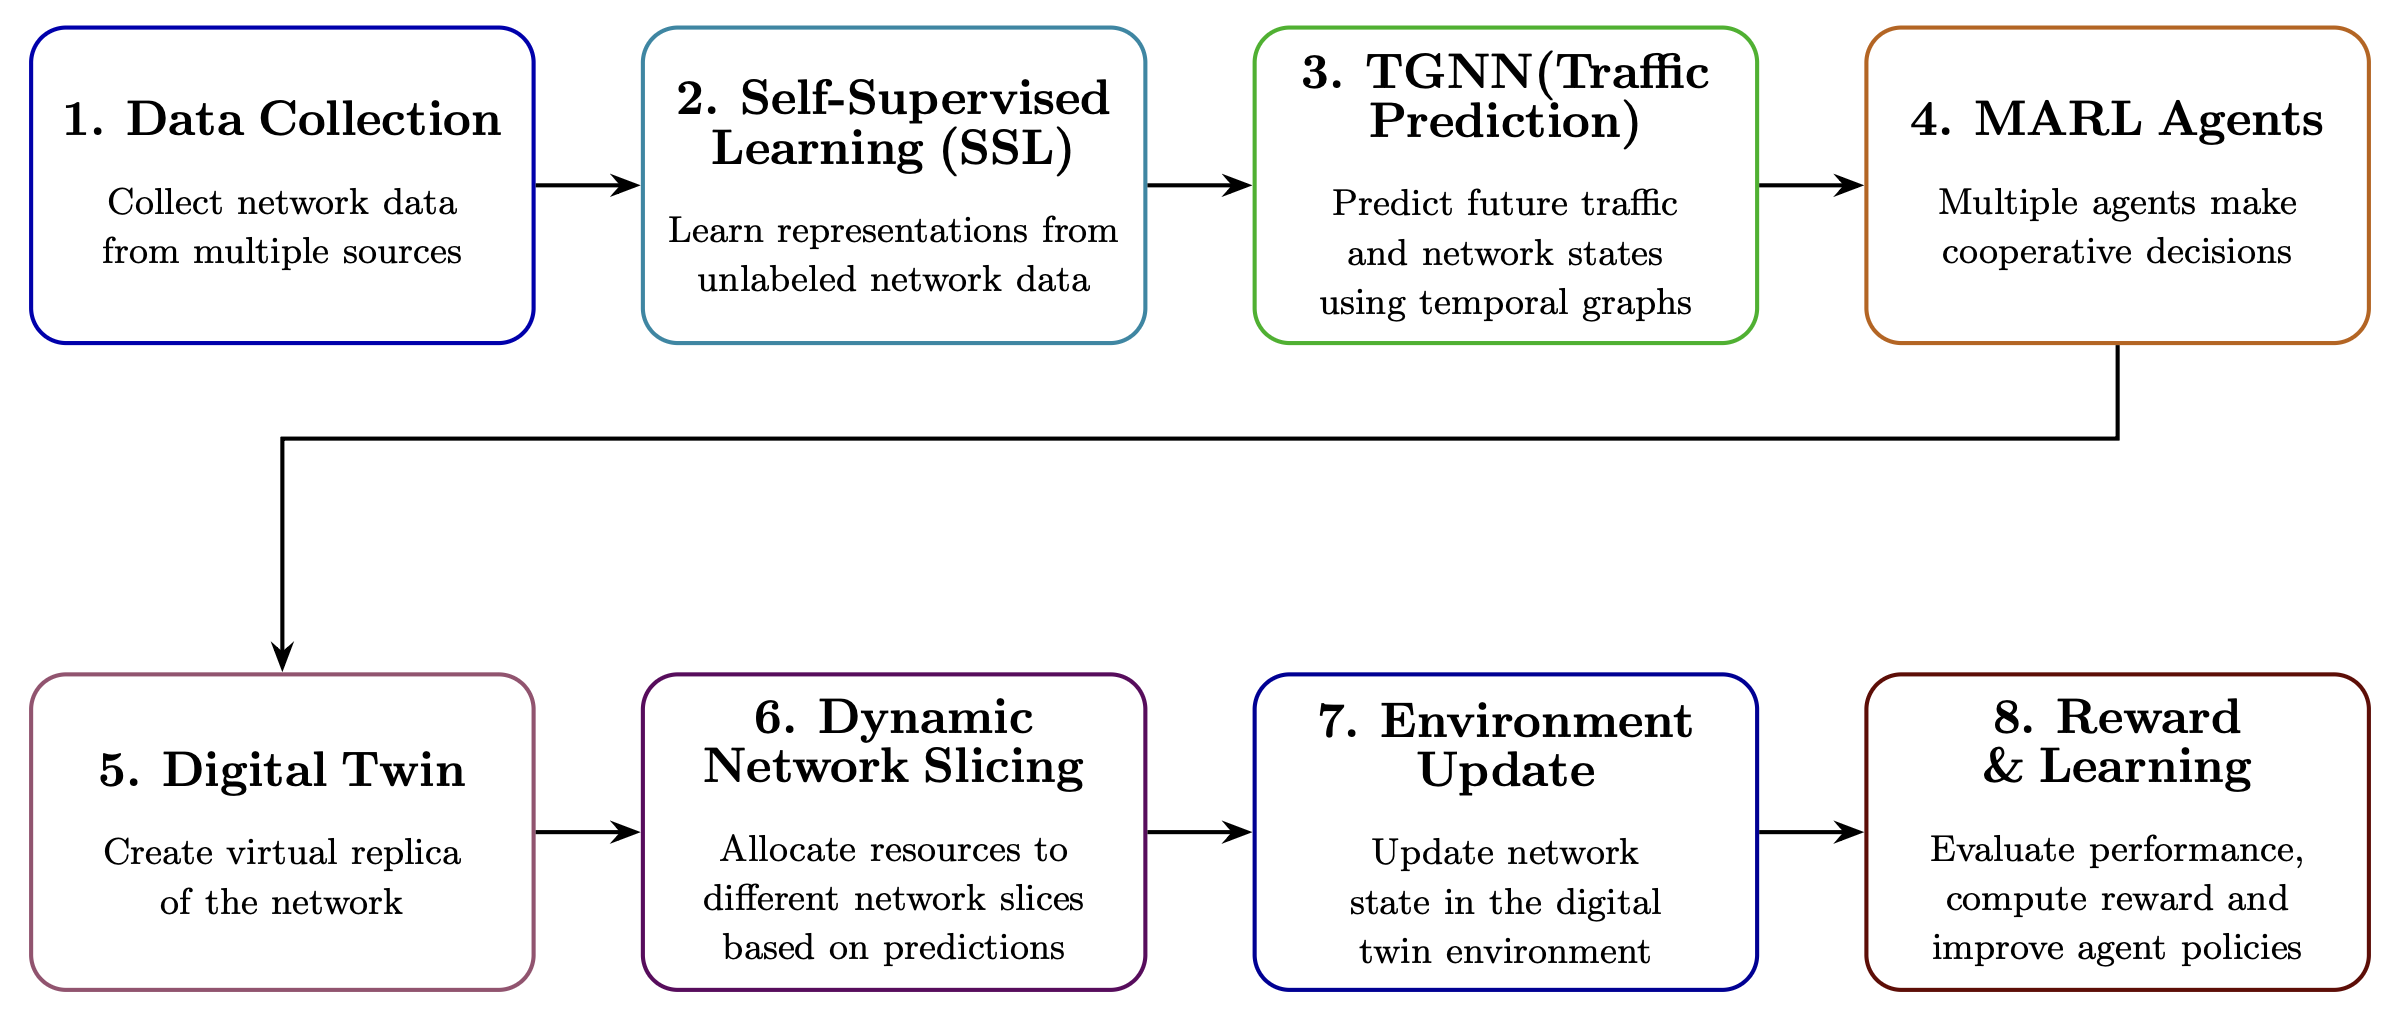
\includegraphics[width=\textwidth]{arch_diag.png}
\caption{Architecture of the proposed system}
\label{fig:arch}
\end{figure}

 
\section{Problem Formulation}
Each cell is controlled by one agent. The agent splits the capacity of its cell into four portions for each of eMBB, URLLC, mMTC and idle and applies the selected portions to the next interval, and so on. Each agent in MARL takes an action only based on 17 local features for their own cell. The load of neighbouring cells diminishes the capacity of a cell (Section~\ref{sec:env}), which means that the decisions of the agents are coupled, and the task is a decentralised multi-agent control problem.

The reward of the agent of cell $i$ in interval $t$ is
\begin{equation}
R_t^{i} = 0.7\,S_t^{i} + 0.3\,F_t^{i} - 0.1\,H_t^{i},
\label{eq:reward}
\end{equation}
where $S_t^{i}$ is a weighted SLA score, $F_t^{i}$ is a fraction of demand that is satisfied and $H_t^{i}$ is a reconfiguration churn. The weights are design choices. The reward therefore favours meeting the SLA targets of the three slices first, then serving demand, and penalises changes of the allocation. During training, each agent's reward is mixed with those of its neighbours (the team reward).

\section{The Unified Slicing Environment}
\label{sec:env}
The environment brings together real traffic on a real spatial layout, per-slice demand, an allocation action, and the resulting QoS, SLA outcome and reward for each cell and each 10-minute interval. It is implemented in the \texttt{src/unified} folder of the project repository. Table~\ref{tab:env} shows which components are real, which are calibrated and which are modelling assumptions.



\begin{table}[h]
\centering
\caption{Components of the unified environment}
\label{tab:env}
\small
\begin{tabular}{|p{3.4cm}|p{2.2cm}|p{9.6cm}|}
\hline
\textbf{Component} & \textbf{Status} & \textbf{Source or rule} \\ \hline
Traffic per cell and interval & Real & Telecom Italia Milan \\ \hline
Topology & Real & Milan grid layout with 4-connected neighbours \\ \hline
Slice demand & Modelled & Internet activity mapped to eMBB, calls to URLLC and SMS to mMTC, scaled so that the 95th percentile of each slice is 80\%, 10\% and 5\% of a 100 Mbps cell \\ \hline
Latency and jitter against load & Calibrated & Curves fitted to the 6G RAN telemetry dataset (30,000 windows) \\ \hline
Inter-cell interference & Modelled & Usable capacity = 100 Mbps / (1 + 0.3 $\times$ mean neighbour load) \\ \hline
Loss and SLA & Rules & Targets given in Table~\ref{tab:sla} \\ \hline
Action & Agent output & Shares of each cell's capacity for eMBB, URLLC, mMTC and idle, applied to the next interval \\ \hline
Reward & Design choice & Equation~(\ref{eq:reward}) \\ \hline
\end{tabular}
\end{table}

\begin{table}[h]
\centering
\caption{SLA targets of the three slices}
\label{tab:sla}
\small
\begin{tabular}{|l|c|c|c|}
\hline
\textbf{Slice} & \textbf{Latency} & \textbf{Jitter} & \textbf{Reliability} \\ \hline
eMBB  & 50 ms  & 20 ms & 0.99 \\ \hline
URLLC & 5 ms   & 1 ms  & 0.99999 \\ \hline
mMTC  & 100 ms & 50 ms & 0.99 \\ \hline
\end{tabular}
\end{table}


The traffic and the grid layout are real. The mapping from activity type to slice and the scaling of each slice to the 100 Mbps cell capacity are assumptions, because the Milan data has no slice information. Latency and jitter as functions of load are the calibrated part and are described next.

\section{Calibration and Realism Check}
To check realism, the eMBB SLA rate of the model was compared with the SLA label of the reference telemetry across fifteen load bins. The deterministic latency model fitted poorly, with a mean difference of 0.086. Adding lognormal spread to the latency, with a single parameter $\sigma = 0.21$, reduced the difference to 0.021. This is not an independent validation, because $\sigma$ was fitted to the same curve.

Two further points limit how far the QoS model can be trusted. It is a calibrated surrogate and not a packet-level simulator, and the reference telemetry used to calibrate it is itself simulated. In addition, the reinforcement learning experiments use the deterministic version of the latency model, without the lognormal spread. Section~\ref{sec:simu5g} compares the model with a packet-level simulator.

\section{Reference Policies}
In addition to the learned controllers, there are three reference policies that are also tested in the environment:
\begin{itemize}
\item \textbf{Equal split}, splits the cell's capacity equally.
\item \textbf{Proportional allocation} means allocating the capacity according to the demand.
\item \textbf{Expert policy}, which allocates sufficient capacity to URLLC and mMTC to maintain their utilisation within the SLA-safe region and the remaining capacity to eMBB.
\end{itemize}
The expert policy is run with three inputs: the current demand, the TGNN forecast of the next interval, and the true demand of the next interval, which is an upper bound. Comparing these three versions measures the value of knowing the next interval without involving a learning method. The rule has two utilisation targets for URLLC and mMTC. Besides the default targets, two tuned versions are used (Chapter~\ref{chap.7}), so that learned controllers are compared with rules that were optimised on the same training days.

\section{Implementation and the Role of the Digital Twin}
The environment and the controllers are implemented in Python with PyTorch, and 25 automated tests pass.

In parallel, a packet-level simulation tool chain was set up: OMNeT++ 6.4.0, INET 4.7.0 and Simu5G 1.7.0 under WSL2. In the reference NR run, a single-cell stand-alone scenario with one gNodeB and one UE, 5 simulated seconds of downlink VoIP were simulated. 28{,}092 events were processed, 93 of 93 packets were delivered, the mean VoIP frame delay was 4.82 ms and the MOS was 4.41 (Figure~\ref{fig:simu5g}). The same tool chain is used for the load sweep of Section~\ref{sec:simu5g}.

The Digital Twin is the unified environment together with the data generated from it (Chapter~\ref{chap.8}). In the early B5G orchestrator an approve-or-reject gate was prototyped, but it could never approve an action because B5G has no telemetry on which to check an SLA. The unified environment has a working gate: it predicts the outcome of a proposed allocation with the environment's QoS model and the TGNN forecast and applies a safe fallback when the proposal looks worse (Section~\ref{sec:gate}).

\begin{figure}[H]
    \centering
    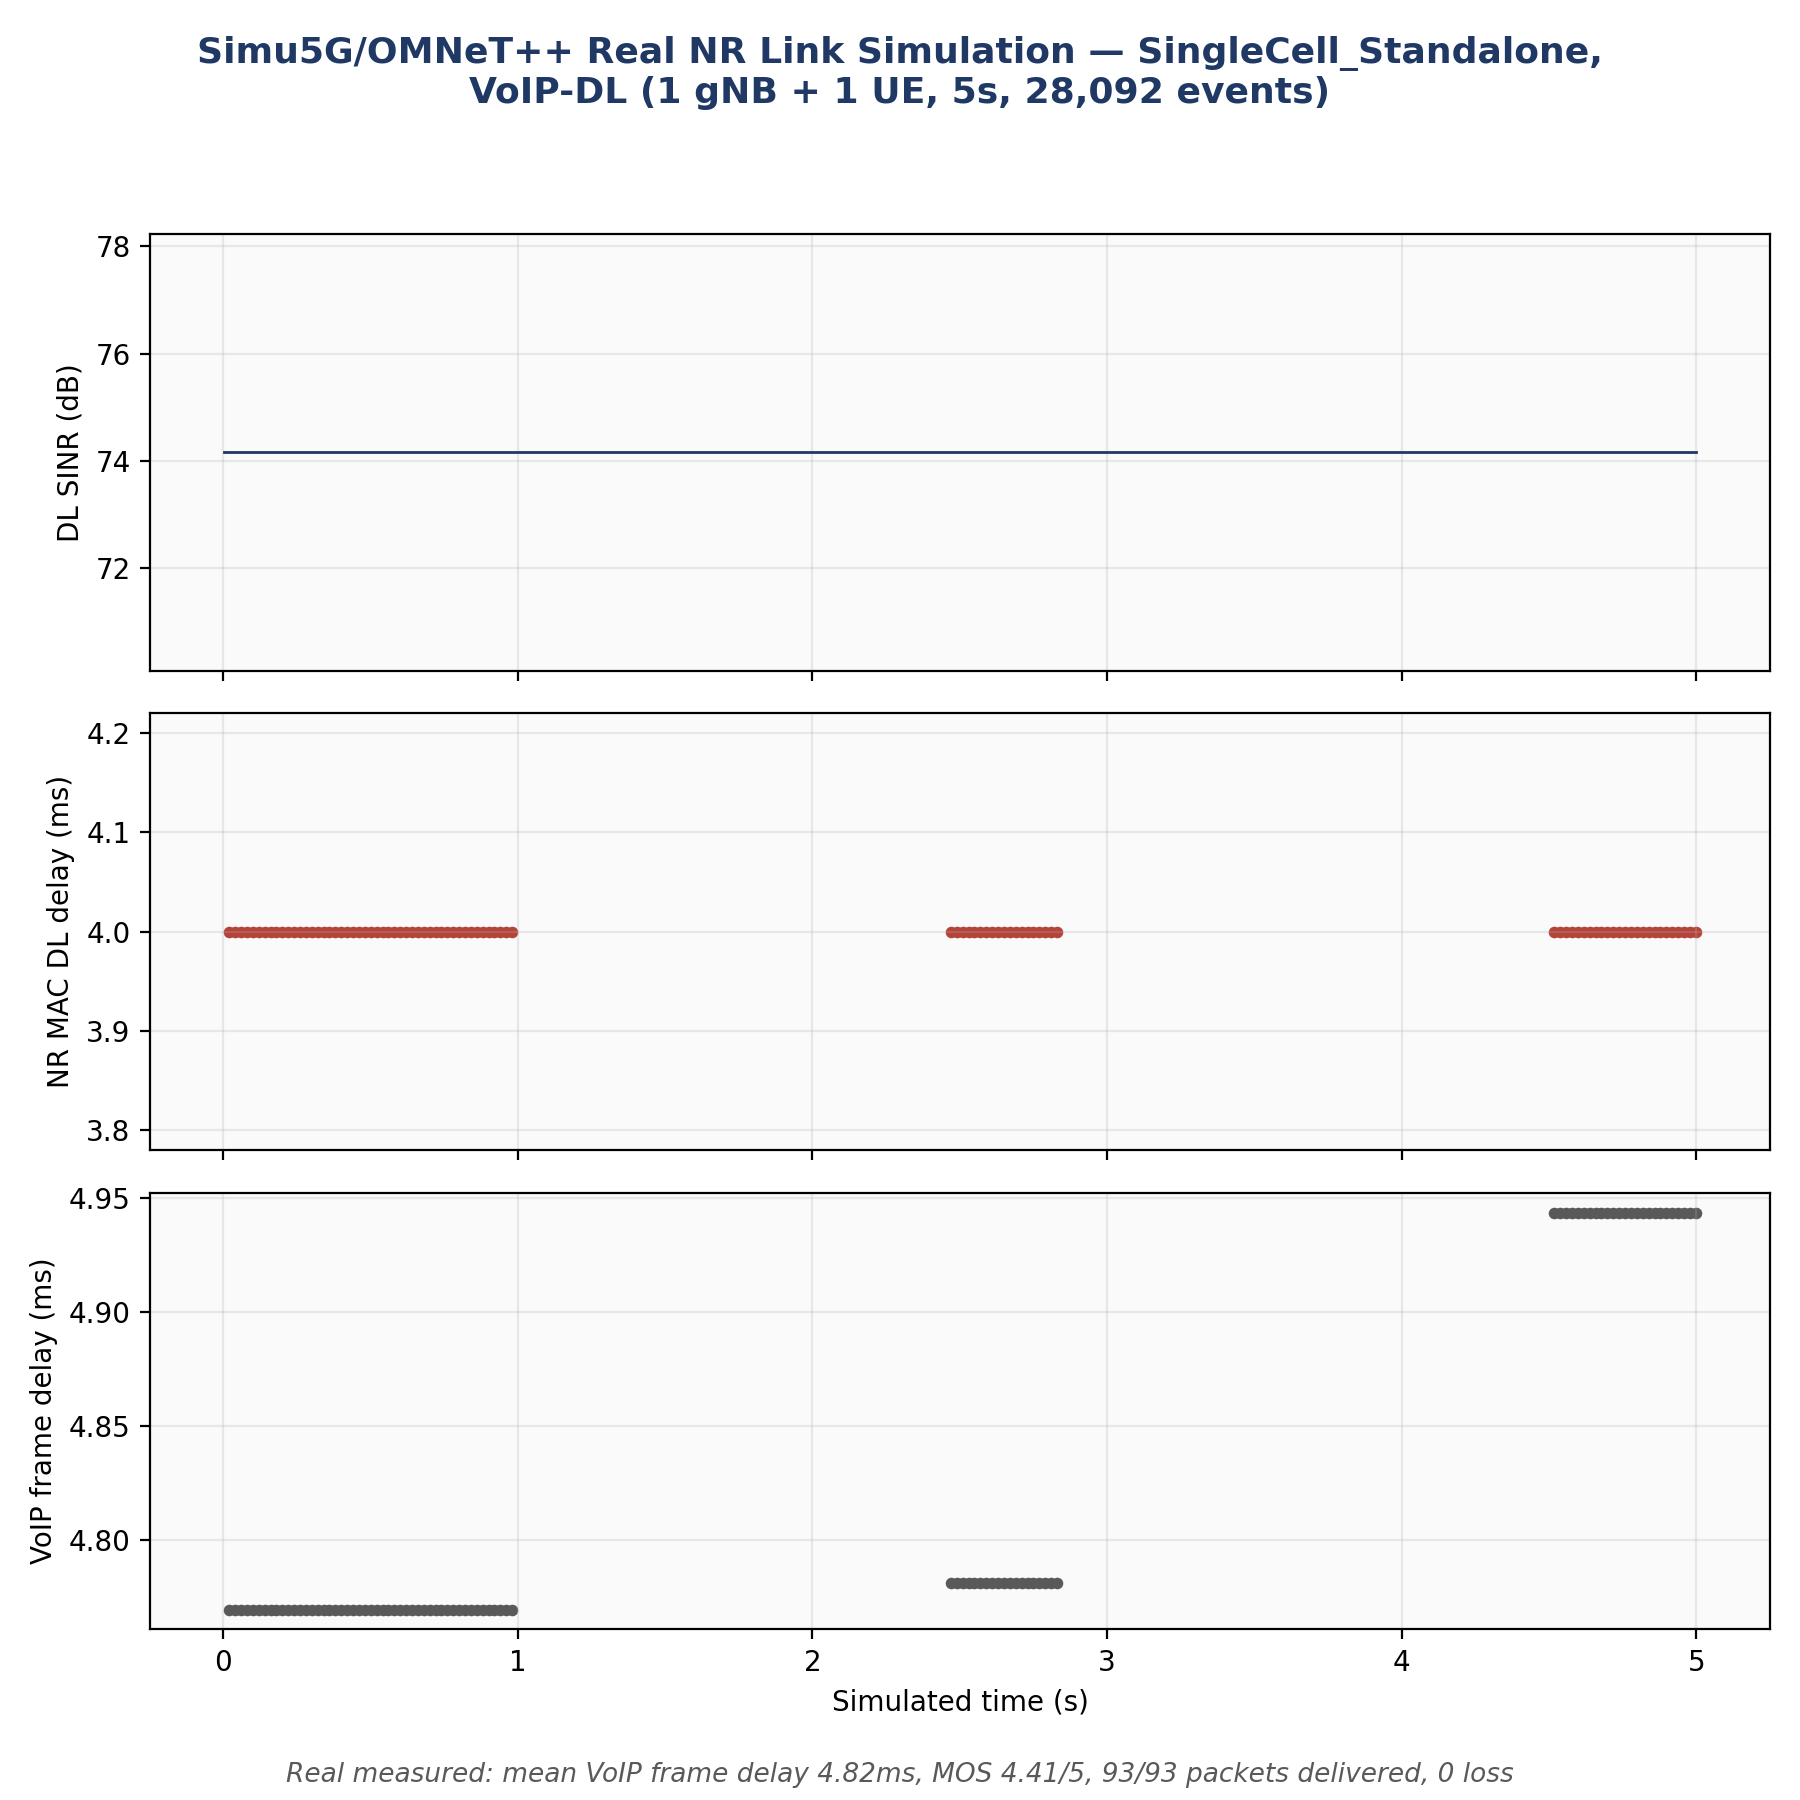
\includegraphics[width=0.75\textwidth,
                     keepaspectratio]{simu5g_ref.png}
    \caption{Reference Simu5G NR run (one gNodeB, one UE, 5 s, downlink VoIP)}
    \label{fig:simu5g}
\end{figure}

\section{Summary}
The unified environment has real traffic and topology from Milan, slice demand, a latency and jitter model calibrated on 6G RAN telemetry, interference from neighbouring cells, and the reward of Equation~(\ref{eq:reward}). It allows forecasting and allocation to be tested together on the same traffic and compared with equal-split, proportional and expert policies, including tuned versions. Its main limit is the surrogate QoS model, which Chapter~\ref{chap.8} compares with a packet-level simulator.
 
\chapter{Self-Supervised Representation Learning}
\label{chap.5}
\section{Motivation and Objective}
Self-supervised learning (SSL) learns representations from network telemetry without needing a label for every observation. The idea in this project was that such representations could feed the later stages, a classifier or the forecaster, and that they would help most when labelled data is scarce. This chapter tests that idea honestly: it describes the encoder, the data problems that first made the results look worse than they were, and a label-efficiency study that asks the question SSL is meant to answer, namely whether pretraining helps when only a few flows are labelled.

\section{Pretext Tasks}
\subsection{First implementation: masked reconstruction}
The first encoder was trained on the 5G-NIDD dataset. Eleven context features (protocol, TCP state, TTL and hop attributes, among others) were treated as categorical variables with an 8-dimensional embedding each. Fourteen volume and rate features (packet and byte counts, mean packet sizes, load and rate) were masked at a ratio of 0.30 and reconstructed from the visible context. The encoder had two linear layers of 128 and 64 units and produced a 64-dimensional embedding; a decoder with a hidden layer of 128 units reconstructed the masked values. The loss is the mean squared error over the masked positions only,
\begin{equation}
\mathcal{L}_{\mathrm{mask}} = \frac{1}{|\mathcal{M}|}\sum_{j\in\mathcal{M}}(\hat{x}_j-x_j)^2 ,
\label{eq:mask_loss}
\end{equation}
where $\mathcal{M}$ is the set of masked positions, $x_j$ the original value and $\hat{x}_j$ the reconstruction. Training used Adam with a learning rate of $10^{-3}$, a batch size of 512 and 10 epochs, on all 1.2 million flows.

\subsection{Re-evaluation: two pretext tasks on cleaned data}
For the final study the pretraining was redone with two standard tabular pretext tasks, using one encoder shape (83 inputs, two hidden layers of 256 units, a 64-dimensional output) so that the comparison between them is fair.
\begin{itemize}
\item \textbf{Masked-feature modelling.} Thirty per cent of the entries of every flow are replaced by the values of the same feature in other flows, and the encoder must reconstruct the original values and also detect which entries were replaced \cite{yoon2020vime}.
\item \textbf{Contrastive learning (SCARF).} Each flow is paired with a copy in which 60\% of the features are replaced by values from random other flows, and a contrastive loss over the batch (temperature 0.5, batch size 512) pulls the two views together \cite{bahri2022scarf}.
\end{itemize}
Both were trained without any label on the 80\% pool of flows kept for training (326{,}924 flows).

\section{Cleaning the Data}
The first evaluation reported a macro-F1 of 0.708. Two data problems explain why that number was so low, and fixing them changed the baseline far more than any SSL variant.
\begin{itemize}
\item \textbf{Duplicate flows.} Of the 1{,}215{,}890 flows in 5G-NIDD, 807{,}235 (66\%) are exact copies, so a random split puts identical flows in the training and the test set. After removing them, 408{,}655 unique flows remain, in nine classes (benign and eight attack types).
\item \textbf{Identifier columns.} The row index, the sequence number and the offset identify a flow's position in the capture and leak its label, so they were removed. The remaining numeric features are heavy-tailed counts, so they were log-scaled, and the categorical features were one-hot encoded, giving 83 inputs.
\end{itemize}
A stratified 80/20 split gives a pretraining pool of 326{,}924 flows and a test set of 81{,}731 flows. A further problem was found earlier: the source file is stored in blocks of identical labels, so a split by position put 99.88\% of one class in the test set and gave an accuracy of about 1\%. The stratified split removed that problem too.

\section{Label-Efficiency Study}
Pretraining is expected to help when labels are scarce, so classifiers were trained with 50, 200, 1{,}000, 5{,}000 and 20{,}000 labelled flows and with all labels. Each budget up to 5{,}000 was repeated with five random label draws (two above that). The classifiers were: logistic regression, a small multilayer perceptron and LightGBM 	te{ke2017lightgbm} on the raw features; logistic regression on the frozen embedding; the pretrained encoder fine-tuned with a classification head; and logistic regression on the raw features concatenated with the embedding. The metric is the macro-averaged F1 over the nine classes.

\begin{table}[htbp]
\centering
\caption{Macro-F1 on 81{,}731 unseen 5G-NIDD flows, by number of labelled flows (mean of five label draws up to 5{,}000 labels, two above)}
\label{tab:ssl_label_efficiency}
\footnotesize
\begin{tabular}{|>{\centering\arraybackslash}p{\dimexpr 0.108\textwidth-2\tabcolsep\relax}|>{\centering\arraybackslash}p{\dimexpr 0.108\textwidth-2\tabcolsep\relax}|>{\centering\arraybackslash}p{\dimexpr 0.108\textwidth-2\tabcolsep\relax}|>{\centering\arraybackslash}p{\dimexpr 0.108\textwidth-2\tabcolsep\relax}|>{\centering\arraybackslash}p{\dimexpr 0.108\textwidth-2\tabcolsep\relax}|>{\centering\arraybackslash}p{\dimexpr 0.108\textwidth-2\tabcolsep\relax}|>{\centering\arraybackslash}p{\dimexpr 0.108\textwidth-2\tabcolsep\relax}|>{\centering\arraybackslash}p{\dimexpr 0.108\textwidth-2\tabcolsep\relax}|>{\centering\arraybackslash}p{\dimexpr 0.108\textwidth-2\tabcolsep\relax}|}
\hline
\textbf{Labels} & \textbf{LGBM raw} & \textbf{MLP raw} & \textbf{Logit raw} & \textbf{Masked emb.} & \textbf{Masked fine-tuned} & \textbf{SCARF emb.} & \textbf{SCARF fine-tuned} & \textbf{Raw + SCARF} \\ \hline
50 & 0.643 & 0.694 & 0.704 & 0.627 & 0.684 & 0.594 & 0.688 & 0.690 \\ \hline
200 & 0.852 & 0.858 & 0.853 & 0.763 & 0.834 & 0.713 & 0.850 & 0.848 \\ \hline
1{,}000 & 0.905 & 0.895 & 0.874 & 0.859 & 0.881 & 0.842 & 0.894 & 0.888 \\ \hline
5{,}000 & 0.919 & 0.911 & 0.909 & 0.901 & 0.898 & 0.880 & 0.901 & 0.915 \\ \hline
20{,}000 & 0.932 & 0.924 & 0.923 & 0.913 & 0.923 & 0.907 & 0.925 & 0.924 \\ \hline
all & 0.936 & 0.925 & 0.926 & 0.912 & 0.927 & 0.910 & 0.929 & 0.926 \\ \hline
\end{tabular}
\end{table}

\begin{figure}[htbp]
\centering
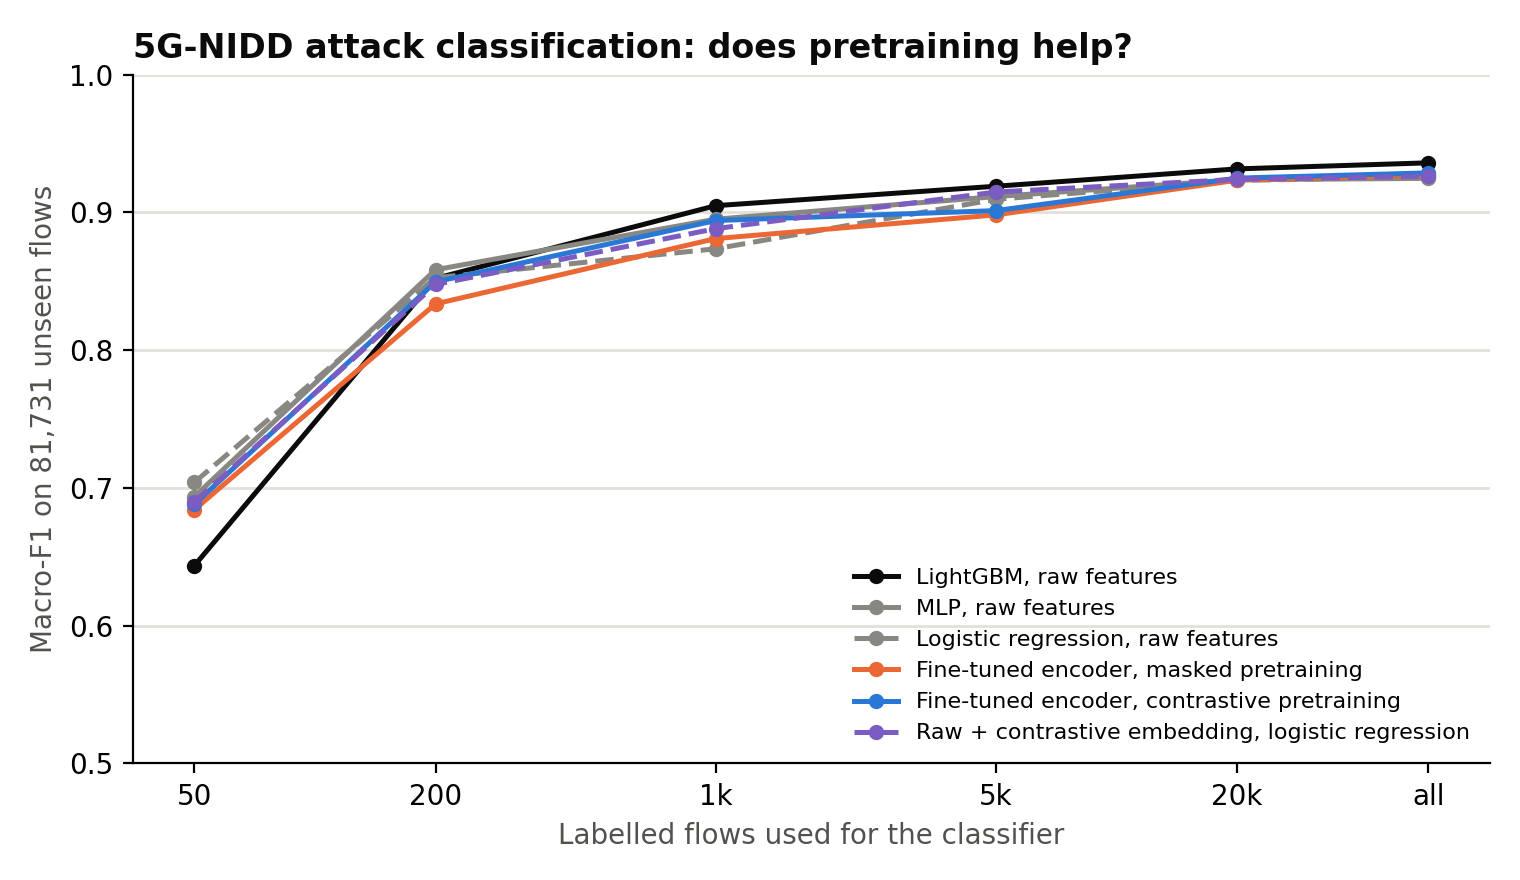
\includegraphics[width=0.9\textwidth,keepaspectratio]{unified_ssl_label_efficiency.png}
\caption{Macro-F1 against the number of labelled flows for raw features and pretrained encoders}
\label{fig:ssl_label_efficiency}
\end{figure}

Three observations follow from Table~\ref{tab:ssl_label_efficiency} and Figure~\ref{fig:ssl_label_efficiency}.
\begin{enumerate}
\item The raw features are already strong. Logistic regression reaches 0.926 and LightGBM 0.936 with all labels, against 0.708 in the first evaluation, so most of the earlier gap came from duplicates and leaked identifiers rather than from the classifier.
\item Pretraining does not beat the best raw-feature model at any budget. With 50 and 200 labels a raw-feature multilayer perceptron or logistic regression is ahead of the fine-tuned encoder (for example 0.694 and 0.704 against 0.688 at 50 labels), and a linear classifier on the frozen embedding alone is clearly worse. With all labels the fine-tuned contrastive encoder ties the same network trained from scratch (0.929 against 0.925) and stays below LightGBM.
\item Adding the embedding to the raw features helps a linear model only a little, by at most 0.014 at 1{,}000 to 5{,}000 labels, and not at all with 20{,}000 or more.
\end{enumerate}
LightGBM is the weakest method at 50 labels because boosted trees need more data, which is why the comparison above is made against the neural and linear raw-feature models as well.

\section{SSL on the Milan Forecast}
\label{sec:milan_ssl}
In the first forecasting experiment (Chapter~\ref{chap.6}) a TGNN fed with 64-dimensional embeddings of Milan traffic features scored the same validation error as one fed with the raw features (0.000616 against 0.000612). That was a single day and a single seed, so it was repeated on the city forecaster. The embedding here is 16-dimensional and describes one cell's input window (the last six intervals of demand, the same time on the previous day, time of day and a weekend flag). An encoder is pretrained without labels by hiding 30\% of the entries of a window and reconstructing them, on windows from the training days only, then frozen and its output is given to the forecaster's output layer. Table~\ref{tab:ssl_milan} gives the outcome. Both variants use the same data, split, scaling and number of training steps; the only difference is the embedding. The pretrained embedding does not help: with it the eMBB improvement is about one percentage point lower (15\% against 16\%), and URLLC and mMTC are within half a point of the raw forecaster. Each variant was trained twice with different seeds, and the run-to-run difference is of the same size as the gap, so we conclude that the embedding adds nothing measurable.

\begin{table}[htbp]
\centering
\caption{City forecaster with and without a pretrained window embedding, improvement over persistence on the held-out week (eMBB / URLLC / mMTC)}
\label{tab:ssl_milan}
\footnotesize
\begin{tabular}{|>{\centering\arraybackslash}p{\dimexpr 0.194\textwidth-2\tabcolsep\relax}|>{\centering\arraybackslash}p{\dimexpr 0.194\textwidth-2\tabcolsep\relax}|>{\centering\arraybackslash}p{\dimexpr 0.194\textwidth-2\tabcolsep\relax}|>{\centering\arraybackslash}p{\dimexpr 0.194\textwidth-2\tabcolsep\relax}|>{\centering\arraybackslash}p{\dimexpr 0.194\textwidth-2\tabcolsep\relax}|}
\hline
\textbf{Forecaster input} & \textbf{Runs} & \textbf{eMBB} & \textbf{URLLC} & \textbf{mMTC} \\ \hline
Raw inputs (the city forecaster as it is) & 2 & +16\% & +32\% & +31\% \\ \hline
Raw inputs + frozen 16-dimensional SSL embedding & 2 & +15\% & +32\% & +31\% \\ \hline
\end{tabular}
\end{table}

\section{Interpretation}
\label{sec:ssl_interpretation}
The finding is the same on both tasks: the raw features already hold what the downstream models need, and masked or contrastive pretraining adds very little. A likely reason is that these are low-dimensional, hand-made features and not raw packets or long sequences. Pretraining is known to pay off on high-dimensional raw inputs, where no one has engineered features. Other work on tabular data reports the same thing, namely that the advantage of pretraining often disappears against well-tuned baselines \cite{rubachev2022revisiting}. We therefore report SSL as a negative result of this project. What this chapter contributes is the cleaned evaluation: de-duplicated data, no leaked columns, a design that varies the number of labels, and strong raw-feature baselines. The SSL stage stays in the pipeline of Chapter~\ref{chap.4} because the literature recommends it, but we do not claim that it improves the forecasts or the allocation.

\chapter{Temporal GNN Traffic Forecasting}
\label{chap.6}
\section{Forecasting Objective}
\label{sec:forecasting_objective}
The forecasting stage predicts the demand of every cell for the next ten minutes, separately for the three slices, using the recent history of the cell and of its neighbours. In the unified environment (Chapter~\ref{chap.4}) the prediction is a vector of three numbers in Mbps per cell. The earlier B5G and NeversNet5G experiments used a similar network to predict throughput, latency and load. A softplus kept the first two non-negative, and a sigmoid kept the load between 0 and 1.

\section{Graph Construction Across Datasets}
\label{sec:graph_construction}
The implementation supports three graph sources.
\paragraph{Milan grid.} The traffic lies on a regular $100\times100$ grid. Each cell is a node joined to its four neighbours, so the graph is the real geographic neighbourhood. The first experiments used a central $20\times20$ block of 400 cells. The final forecaster covers all 10{,}000 cells.
\paragraph{NeversNet5G.} Here the graph snapshots come from event-driven UE telemetry and keep the identities of the UEs and gNodeBs and how they relate over time. The 64-dimensional SSL embeddings we exported are aligned with the graph timestamps. When a gNodeB has no embedding of its own, we average the embeddings of the UEs connected to it.
\paragraph{B5G topology.} The B5G pipeline uses the graph, the routing matrix and the slice configuration that come with the dataset. It replays recorded samples instead of running an online simulator, and the recorded delta value serves as the reward.

\section{GraphSAGE--GRU Architecture}
\label{sec:graphsage_gru}
At every time step two GraphSAGE layers combine each node's features with the mean of its neighbours' features,
\begin{equation}
h_v^{(l+1)} = \sigma\!\left(W^{(l)}\left[h_v^{(l)} \,\Vert\, \operatorname{mean}_{u\in\mathcal{N}(v)} h_u^{(l)}\right]\right),
\label{eq:graphsage_update}
\end{equation}
where $h_v^{(l)}$ is the representation of node $v$ at layer $l$, $\mathcal{N}(v)$ its neighbours, $W^{(l)}$ a weight matrix and $\sigma$ an activation \cite{hamilton2017}. The sequence of spatial representations over the observation window is fed to a GRU cell, and the final hidden state is used to predict the next interval. The temporal part is a plain \texttt{GRUCell} over the output of PyTorch Geometric's \texttt{SAGEConv}, not the graph-convolutional GRU of the original design, because \texttt{torch\_sparse} did not install on the Windows development machine.

\section{First Experiments on the Milan Block}
\label{sec:milan_tgnn_experiments}
The first experiment used 400 cells over one day of 144 ten-minute steps, with a window of five steps (111 training and 28 validation windows) and 25 epochs of Adam at a learning rate of 0.0005. We compared the TGNN with persistence and with the training mean.
\begin{table}[htbp]
\centering
\caption{First Milan block experiment (one day, 400 cells, one seed)}
\label{tab:milan_forecasting}
\begin{tabular}{|l|c|}
\hline
\textbf{Model} & \textbf{Validation MSE} \\ \hline
GraphSAGE--GRU TGNN & 0.0006160 \\ \hline
Persistence & 0.0007196 \\ \hline
Training-mean predictor & 0.0063946 \\ \hline
\end{tabular}
\end{table}
The TGNN was about 14\% better than persistence. With only one day and one seed this shows that the model can learn the short-term pattern, not that it generalises. Feeding the five raw features in place of the SSL embeddings gave 0.0006122, so the embedding added nothing (Chapter~\ref{chap.5}).

\begin{figure}[htbp]
\centering
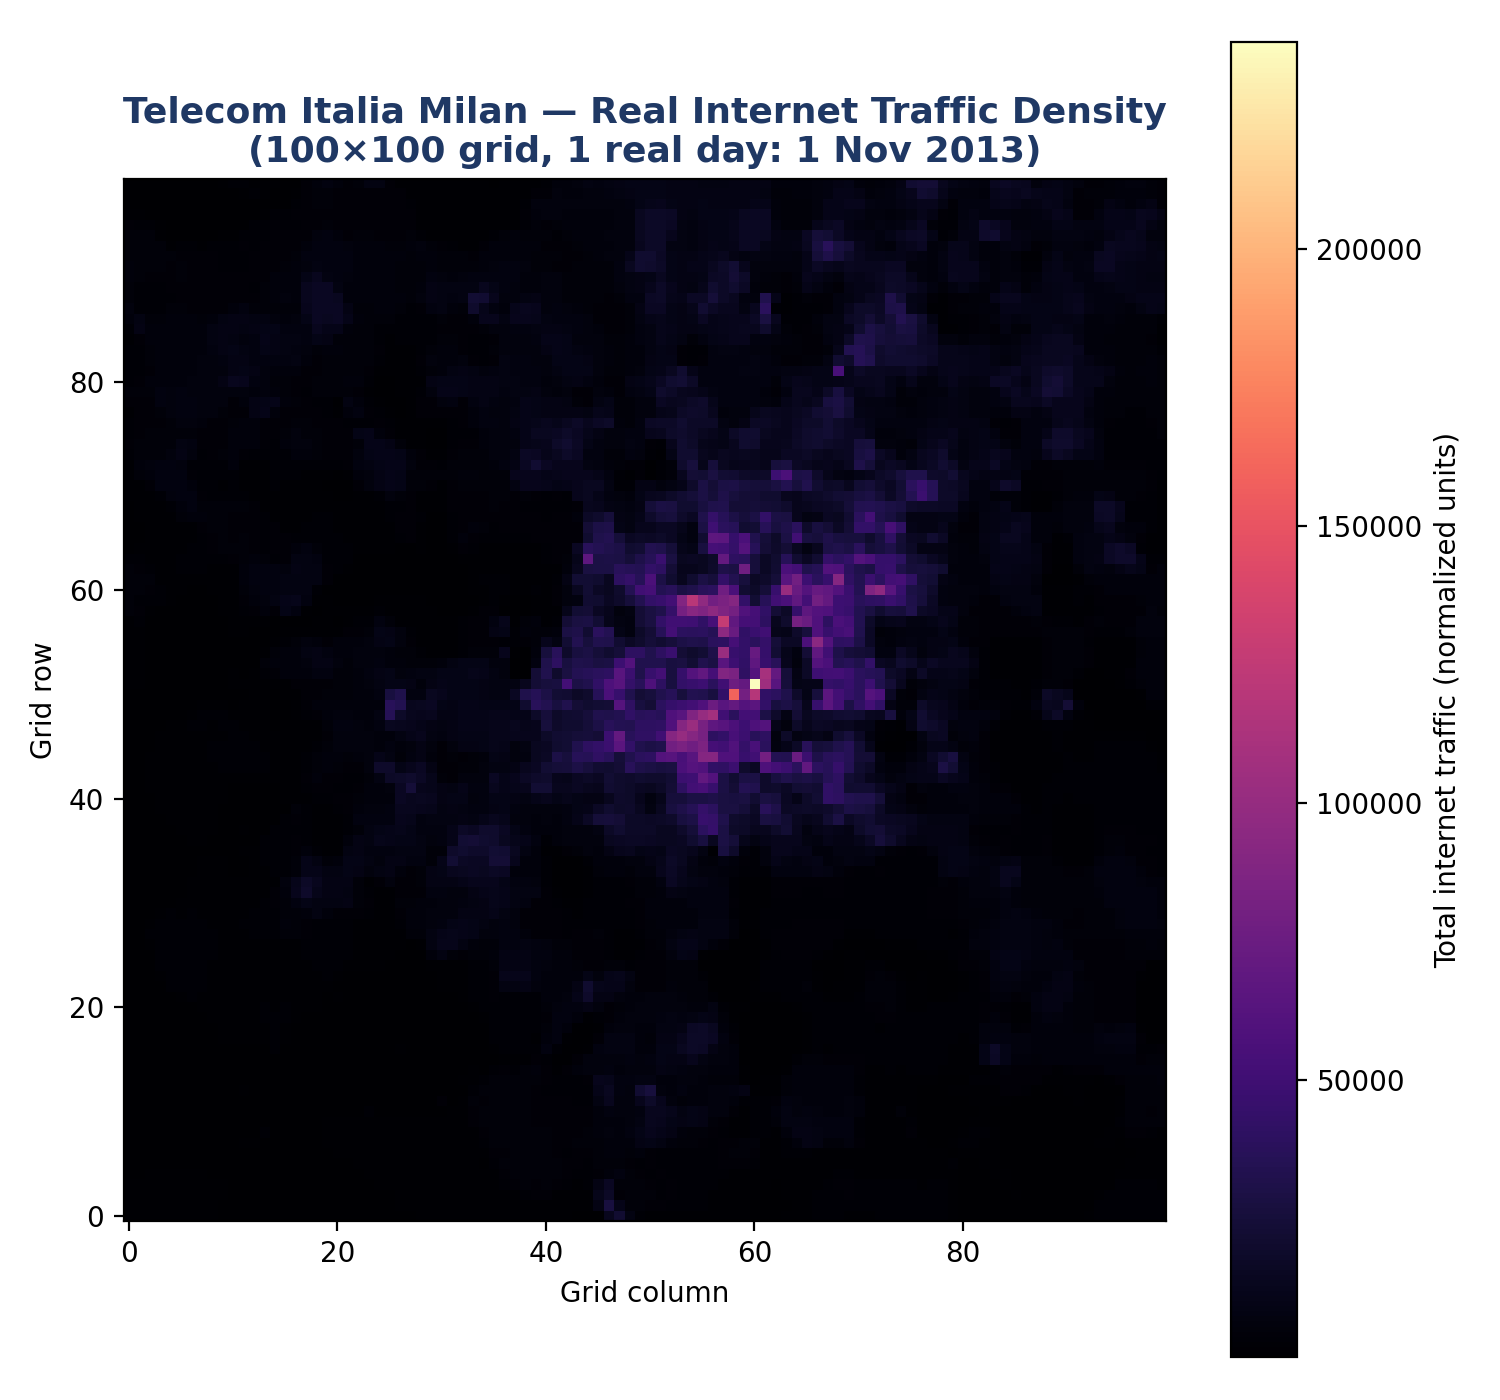
\includegraphics[width=0.55\textwidth,keepaspectratio]{milan_traffic_heatmap.png}
\caption{Real traffic on the Milan grid}
\label{fig:milan_heatmap}
\end{figure}\begin{figure}[htbp]
\centering
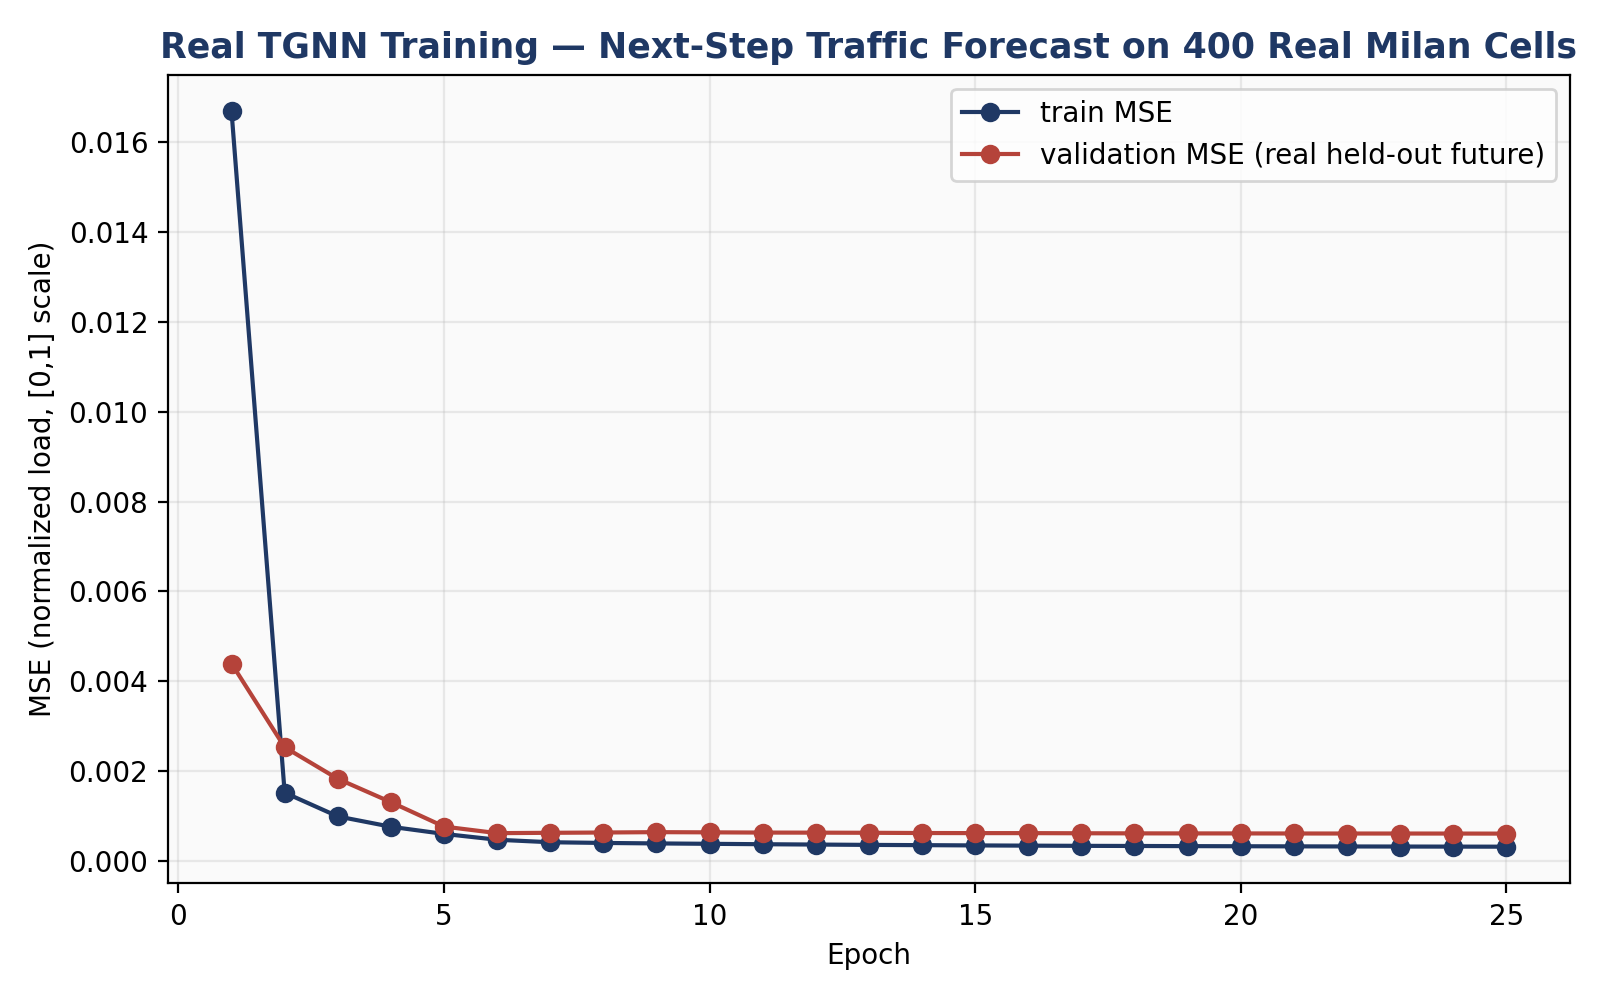
\includegraphics[width=0.8\textwidth,keepaspectratio]{tgnn_milan_forecast_training.png}
\caption{Training and validation error of the first Milan forecaster}
\label{fig:tgnn_first_training}
\end{figure}

\section{City-Wide Generalisation Failure}
\label{sec:city_generalisation_failure}
We applied the forecaster trained on the 100 central cells to all 10{,}000 cells of the city, and it failed on the quiet ones. It had only seen the dense centre, so it had learned that traffic is heavy, and it over-predicted the suburbs by about 6 Mbps on average. On the 9{,}600 outer cells its eMBB error was 10.8 times that of persistence.

\begin{table}[htbp]
\centering
\caption{City-wide evaluation of the forecaster trained on the 100 central cells only (eMBB mean squared error, Mbps$^2$, two held-out days)}
\label{tab:block_city_generalisation}
\footnotesize
\begin{tabular}{|>{\centering\arraybackslash}p{\dimexpr 0.300\textwidth-2\tabcolsep\relax}|>{\centering\arraybackslash}p{\dimexpr 0.170\textwidth-2\tabcolsep\relax}|>{\centering\arraybackslash}p{\dimexpr 0.170\textwidth-2\tabcolsep\relax}|>{\centering\arraybackslash}p{\dimexpr 0.170\textwidth-2\tabcolsep\relax}|}
\hline
\textbf{Region} & \textbf{TGNN} & \textbf{Persistence} & \textbf{TGNN error relative to persistence} \\ \hline
100-cell block & 54.00 & 61.23 & 0.9$\times$ \\ \hline
300-cell core ring & 61.59 & 57.10 & 1.1$\times$ \\ \hline
9{,}600 outer cells & 47.54 & 4.38 & 10.8$\times$ \\ \hline
All 10{,}000 cells & 48.03 & 6.53 & 7.4$\times$ \\ \hline
\end{tabular}
\end{table}

This is a level-bias and spatial-coverage problem: a model that has never seen a quiet cell cannot predict one.

\section{The Corrected City Forecaster}
\label{sec:corrected_city_forecaster}
The architecture was kept and the training was changed in four ways.
\begin{enumerate}
\item \textbf{Per-cell scaling.} We divide the demand of each cell by its own typical level (the median over the training days of its daily 95th percentile, with a floor of 1\% of the city-wide value). The model then learns the shape of the change and not the level.
\item \textbf{Spatial sampling.} Every training step uses a randomly placed $32\times32$ patch of the grid, so central, suburban and intermediate traffic are all seen.
\item \textbf{More data and better inputs.} The model trains on 39 real days. Days 5 and 6 are left out because we use them later for tests, and days 41 to 44 serve as validation for choosing the epoch. Each step also sees the demand of the cell at the same time on the previous day, which is known in advance, plus a time-of-day encoding and a weekend flag.
\item \textbf{No output ceiling.} The old output layer passed the mMTC prediction through a sigmoid, which capped it at the usual level of the cell. The new head predicts a correction to the last observed demand with no upper limit, so spikes can be forecast.
\end{enumerate}
We test the model on a held-out week, 16 to 22 December 2013 (days 45 to 51), over every cell and against persistence. Table~\ref{tab:city_forecaster_improvement} gives the improvement in mean squared error.

\begin{table}[htbp]
\centering
\caption{Improvement over persistence on the held-out week, 16--22 December 2013 (eMBB / URLLC / mMTC)}
\label{tab:city_forecaster_improvement}
\footnotesize
\begin{tabular}{|>{\centering\arraybackslash}p{\dimexpr 0.300\textwidth-2\tabcolsep\relax}|>{\centering\arraybackslash}p{\dimexpr 0.170\textwidth-2\tabcolsep\relax}|>{\centering\arraybackslash}p{\dimexpr 0.170\textwidth-2\tabcolsep\relax}|}
\hline
\textbf{Region} & \textbf{Trained on 5 days} & \textbf{Trained on 39 days} \\ \hline
100-cell block & -12\% / +17\% / +21\% & +21\% / +36\% / +35\% \\ \hline
300-cell core ring & -49\% / +8\% / +7\% & +15\% / +33\% / +32\% \\ \hline
9{,}600 outer cells & -34\% / +9\% / +5\% & +18\% / +34\% / +31\% \\ \hline
All 10{,}000 cells & -34\% / +9\% / +7\% & +18\% / +33\% / +31\% \\ \hline
\end{tabular}
\end{table}

\begin{figure}[htbp]
\centering
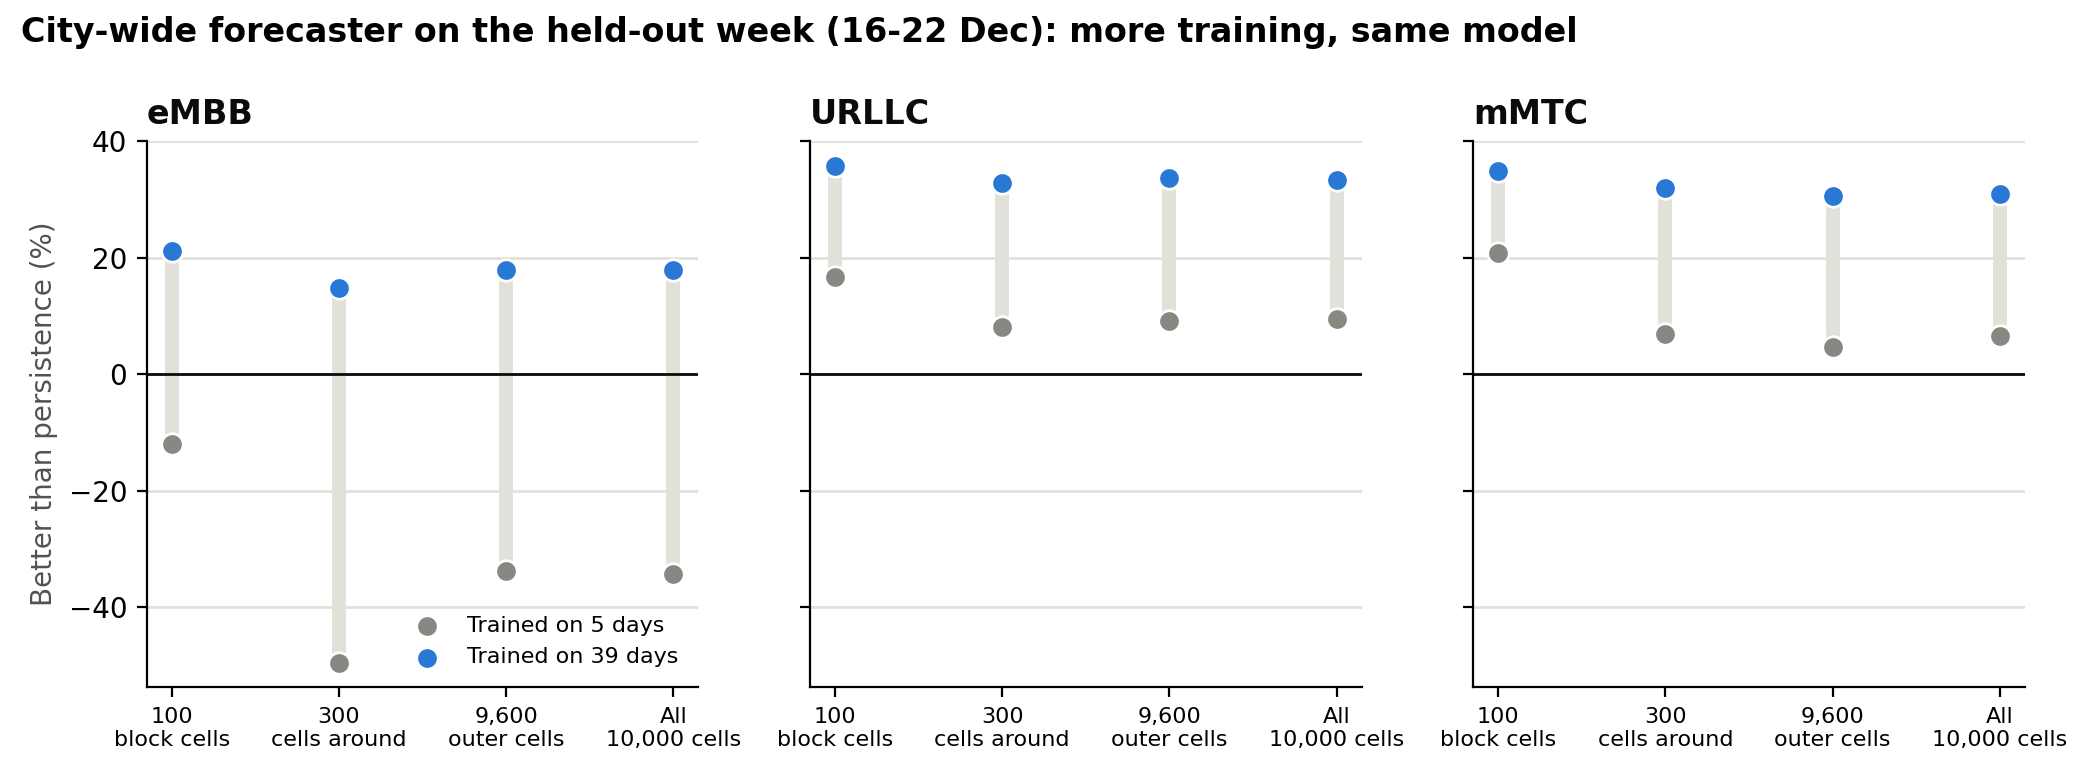
\includegraphics[width=\textwidth,keepaspectratio]{unified_forecast_city.png}
\caption{City-wide forecaster on the held-out week: five days of training against 39 days}
\label{fig:city_forecaster}
\end{figure}

The retrained forecaster beats persistence in every region and for every slice, including the 100 central cells where the earlier model was trained. The five-day version of the same model is worse than persistence on eMBB in this week. So the amount of training data, and not the architecture, was the main limit.

Table~\ref{tab:forecast_baselines} compares the model with two seasonal baselines. At a horizon of ten minutes persistence is very hard to beat. The value at the same time on the previous day gives 8.1 times the eMBB error of persistence, and the average for that time of day gives 13.6 times. Persistence is therefore the right baseline to beat.

\begin{table}[htbp]
\centering
\caption{Mean squared error of simple baselines and the TGNN on all 10{,}000 cells (Mbps$^2$), held-out week}
\label{tab:forecast_baselines}
\footnotesize
\begin{tabular}{|>{\centering\arraybackslash}p{\dimexpr 0.300\textwidth-2\tabcolsep\relax}|>{\centering\arraybackslash}p{\dimexpr 0.170\textwidth-2\tabcolsep\relax}|>{\centering\arraybackslash}p{\dimexpr 0.170\textwidth-2\tabcolsep\relax}|>{\centering\arraybackslash}p{\dimexpr 0.170\textwidth-2\tabcolsep\relax}|}
\hline
\textbf{Forecaster} & \textbf{eMBB} & \textbf{URLLC} & \textbf{mMTC} \\ \hline
Repeat the last value (persistence) & 1.449 & 0.127 & 0.061 \\ \hline
Same time on the previous day & 11.799 & 0.666 & 0.193 \\ \hline
Average for that time of day & 19.736 & 0.522 & 0.152 \\ \hline
TGNN, trained on 39 days & 1.190 & 0.084 & 0.042 \\ \hline
\end{tabular}
\end{table}

\section{Limitations of the Forecasting Study}
\label{sec:pending_forecasting_experiments}
We trained each forecaster once, so we have no estimate of the variation between seeds. We also did not separate the contributions of per-cell scaling, patch sampling, the extra inputs and the graph aggregation, and we have no graph-free baseline (a GRU on each cell alone) or published spatio-temporal baselines such as STGCN. These tests would show which part of the model does the work, and they are listed as future work in Chapter~\ref{chap.10}. The value of the forecast to the controllers is measured in Chapter~\ref{chap.8}.

\chapter{MARL for Slice Allocation}
\label{chap.7}
\section{Allocation Problem}
\label{sec:allocation_problem}
The last learned component shares the capacity of each cell between the eMBB, URLLC and mMTC slices. Every cell has its own agent. The agent sees 17 local quantities: the demand, utilisation and QoS of each slice, its previous allocation, the time of day, and the forecast when one is given. It outputs four non-negative numbers, and a softmax turns them into the shares of eMBB, URLLC, mMTC and idle capacity. The environment of Chapter~\ref{chap.4} then works out the QoS, the SLA outcomes and the reward. The cells affect each other only through interference, since the usable capacity of a cell drops when its neighbours are loaded.

\section{Scalable MARL Design}
\label{sec:scalable_marl}
All cells share one actor, a network with 19{,}332 parameters that maps the observation of a cell to its allocation. The actor never looks at other cells, so the same copy works at any network size. Training uses a centralised critic that looks at the neighbourhood: it takes the observation and action of a cell together with the mean observation and mean action of its grid neighbours. The reward of each agent also contains a share of its neighbours' rewards, which pushes the agents to coordinate locally.

The learning algorithm is an actor--critic in the style of MADDPG \cite{lowe2017}. It uses a replay buffer of 50{,}000 transitions, a discount factor of 0.9, soft target updates with $\tau=0.01$, learning rates of $3\times10^{-4}$ for the actor and $10^{-3}$ for the critic, and exploration noise added in logit space. The earlier B5G trainer used the observed reward as a one-step target, because its offline samples are single decisions and not interactions with a simulator.

\section{Evaluation Protocol}
\label{sec:marl_protocol}
Every result in this chapter uses the same protocol. Agents train on days 1 to 40 of the recorded data. Days 41 to 44 are only used to pick a checkpoint or tune a rule. The test is the held-out week of 16 to 22 December 2013, with one reward per day, and each table entry is the mean of those seven days. We compare two controllers day by day and quote a 95\% interval on the mean difference, using a $t$ value for six degrees of freedom. Consecutive days are not independent, so the intervals only describe how much the days of this one week vary; they say nothing about another week or another city. Learned policies are also averaged over several seeds, and every table gives the number of seeds.

\section{MARL versus a Single Central Agent}
\label{sec:marl_comparison}
The first question is whether splitting the problem into local agents matters. A single central agent sees the observations of all cells and outputs all the allocations at once. We trained it with two learning rates, on the same data, reward and number of episodes. Table~\ref{tab:marl_scaling} shows the result at a budget of 1{,}000 episodes.

\begin{table}[htbp]
\centering
\caption{Held-out week reward at a training budget of 1{,}000 episodes (mean over seeds, number of seeds in brackets)}
\label{tab:marl_scaling}
\footnotesize
\begin{tabular}{|>{\centering\arraybackslash}p{\dimexpr 0.121\textwidth-2\tabcolsep\relax}|>{\centering\arraybackslash}p{\dimexpr 0.121\textwidth-2\tabcolsep\relax}|>{\centering\arraybackslash}p{\dimexpr 0.121\textwidth-2\tabcolsep\relax}|>{\centering\arraybackslash}p{\dimexpr 0.121\textwidth-2\tabcolsep\relax}|>{\centering\arraybackslash}p{\dimexpr 0.121\textwidth-2\tabcolsep\relax}|>{\centering\arraybackslash}p{\dimexpr 0.121\textwidth-2\tabcolsep\relax}|>{\centering\arraybackslash}p{\dimexpr 0.121\textwidth-2\tabcolsep\relax}|>{\centering\arraybackslash}p{\dimexpr 0.121\textwidth-2\tabcolsep\relax}|}
\hline
\textbf{Cells} & \textbf{Shared MARL} & \textbf{Single agent (lr $10^{-4}$ / $3\times10^{-4}$)} & \textbf{Equal split} & \textbf{Expert, current} & \textbf{Expert, forecast} & \textbf{Expert, forecast, tuned} & \textbf{Expert, true next} \\ \hline
9 & $0.926\pm0.005$ (2) & 0.433 / 0.442 & 0.785 & 0.794 & 0.825 & 0.909 & 0.945 \\ \hline
25 & $0.833\pm0.086$ (2) & 0.337 / 0.329 & 0.750 & 0.775 & 0.804 & 0.877 & 0.920 \\ \hline
100 & 0.857 (1) & 0.284 / 0.267 & 0.735 & 0.765 & 0.794 & 0.865 & 0.908 \\ \hline
\end{tabular}
\end{table}

\begin{figure}[htbp]
\centering
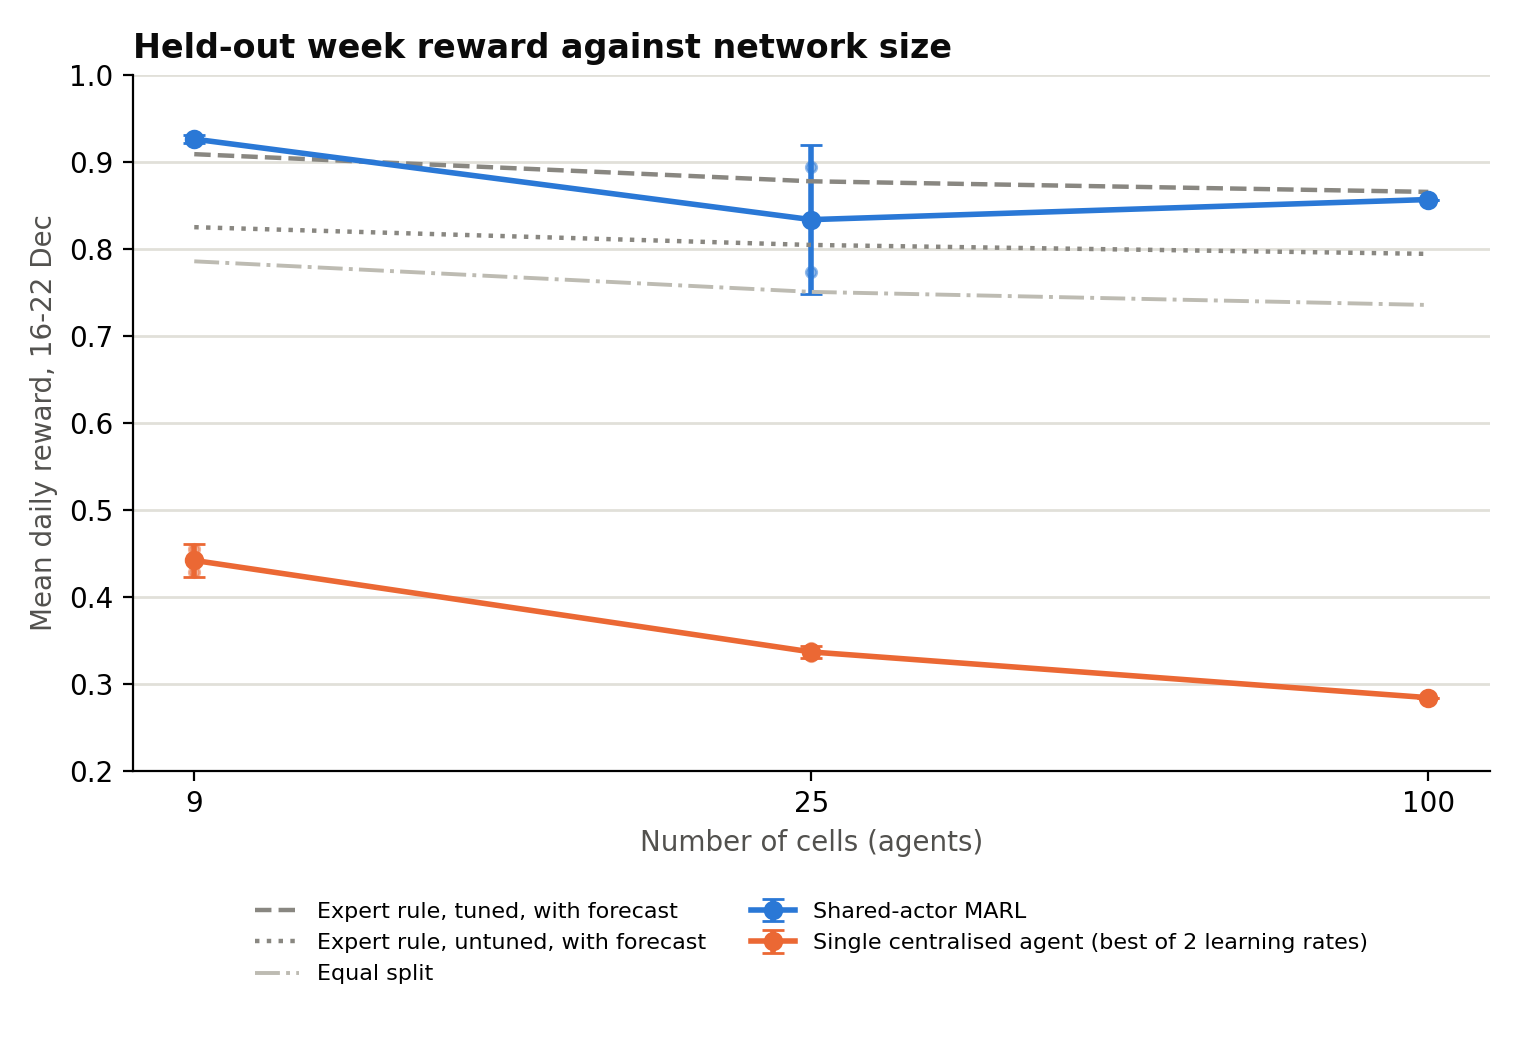
\includegraphics[width=0.85\textwidth,keepaspectratio]{unified_marl_vs_single.png}
\caption{Reward against network size: shared MARL, the single agent and the reference rules}
\label{fig:marl_scaling}
\end{figure}

The shared actor keeps both its size and its reward as the network grows. The central actor, in contrast, grows from 114{,}468 to 604{,}048 parameters (Table~\ref{tab:marl_parameter_growth}) and its reward falls from about 0.43 to 0.27--0.28. This supports the split into local agents. The central agent has to learn a very large action space from one learning step per episode step, and in our runs its reward went down during training instead of up. So the result tells us that this central baseline works badly, not that every centralised design would. Sharing parameters is the natural way to keep the problem manageable, and that is the point of the comparison.

\begin{table}[htbp]
\centering
\caption{Policy size as the network grows}
\label{tab:marl_parameter_growth}
\footnotesize
\begin{tabular}{|>{\centering\arraybackslash}p{\dimexpr 0.300\textwidth-2\tabcolsep\relax}|>{\centering\arraybackslash}p{\dimexpr 0.170\textwidth-2\tabcolsep\relax}|>{\centering\arraybackslash}p{\dimexpr 0.170\textwidth-2\tabcolsep\relax}|>{\centering\arraybackslash}p{\dimexpr 0.170\textwidth-2\tabcolsep\relax}|}
\hline
\textbf{Cells} & \textbf{Shared actor parameters} & \textbf{Single-agent actor parameters} & \textbf{Central input / output size} \\ \hline
9 & 19{,}332 & 114{,}468 & 153 / 36 \\ \hline
25 & 19{,}332 & 200{,}548 & 425 / 100 \\ \hline
100 & 19{,}332 & 604{,}048 & 1700 / 400 \\ \hline
\end{tabular}
\end{table}

\section{Comparison with Properly Tuned Rules}
\label{sec:marl_vs_tuned}
A learned controller should also be compared with the strongest simple one, not only with an equal split. The expert rule gives URLLC and mMTC enough capacity to hold their utilisation at a target, and the rest to eMBB. Its default targets were picked by hand, so we built two tuned versions that use the training days only.
\begin{itemize}
\item \textbf{Simple tuned rule.} Two utilisation targets, one for URLLC and one for mMTC, are chosen by grid search on the training days. At 25 cells the search picks 0.4 and 0.4, and the held-out reward of the forecast-fed rule rises from 0.804 to 0.878.
\item \textbf{Rich tuned rule.} The targets are chosen separately for each four-hour block of the day and each of three cell classes (by traffic level), 18 pairs in total.
\end{itemize}
Table~\ref{tab:marl_scaling} shows that at 1{,}000 episodes the shared MARL controller is clearly better than the untuned rules, but at 25 and 100 cells it loses to the simple tuned rule. We therefore moved to a longer protocol: 4{,}000 episodes, the checkpoint with the best validation reward, and an average of the actors from several seeds in logit space. Table~\ref{tab:marl_long} gives the result.

\begin{table}[htbp]
\centering
\caption{Long protocol (4{,}000 episodes, checkpoint chosen on validation days, actors averaged in logit space) against the tuned expert rules, held-out week (difference in reward, 95\% CI, days better out of 7)}
\label{tab:marl_long}
\footnotesize
\begin{tabular}{|>{\centering\arraybackslash}p{\dimexpr 0.139\textwidth-2\tabcolsep\relax}|>{\centering\arraybackslash}p{\dimexpr 0.139\textwidth-2\tabcolsep\relax}|>{\centering\arraybackslash}p{\dimexpr 0.139\textwidth-2\tabcolsep\relax}|>{\centering\arraybackslash}p{\dimexpr 0.139\textwidth-2\tabcolsep\relax}|>{\centering\arraybackslash}p{\dimexpr 0.139\textwidth-2\tabcolsep\relax}|>{\centering\arraybackslash}p{\dimexpr 0.139\textwidth-2\tabcolsep\relax}|>{\centering\arraybackslash}p{\dimexpr 0.139\textwidth-2\tabcolsep\relax}|}
\hline
\textbf{Cells} & \textbf{MARL (actors)} & \textbf{Simple tuned expert} & \textbf{MARL minus simple} & \textbf{Rich tuned expert} & \textbf{MARL minus rich} & \textbf{True-next oracle} \\ \hline
9 & 0.933 (3) & 0.909 & +0.024 $\pm$ 0.004 (7/7) & 0.928 & +0.005 $\pm$ 0.004 (6/7) & 0.945 \\ \hline
25 & 0.904 (3) & 0.877 & +0.026 $\pm$ 0.005 (7/7) & 0.899 & +0.005 $\pm$ 0.003 (7/7) & 0.920 \\ \hline
100 & 0.888 (1) & 0.865 & +0.023 $\pm$ 0.006 (7/7) & 0.887 & +0.001 $\pm$ 0.003 (3/7) & 0.908 \\ \hline
\end{tabular}
\end{table}

\begin{figure}[htbp]
\centering
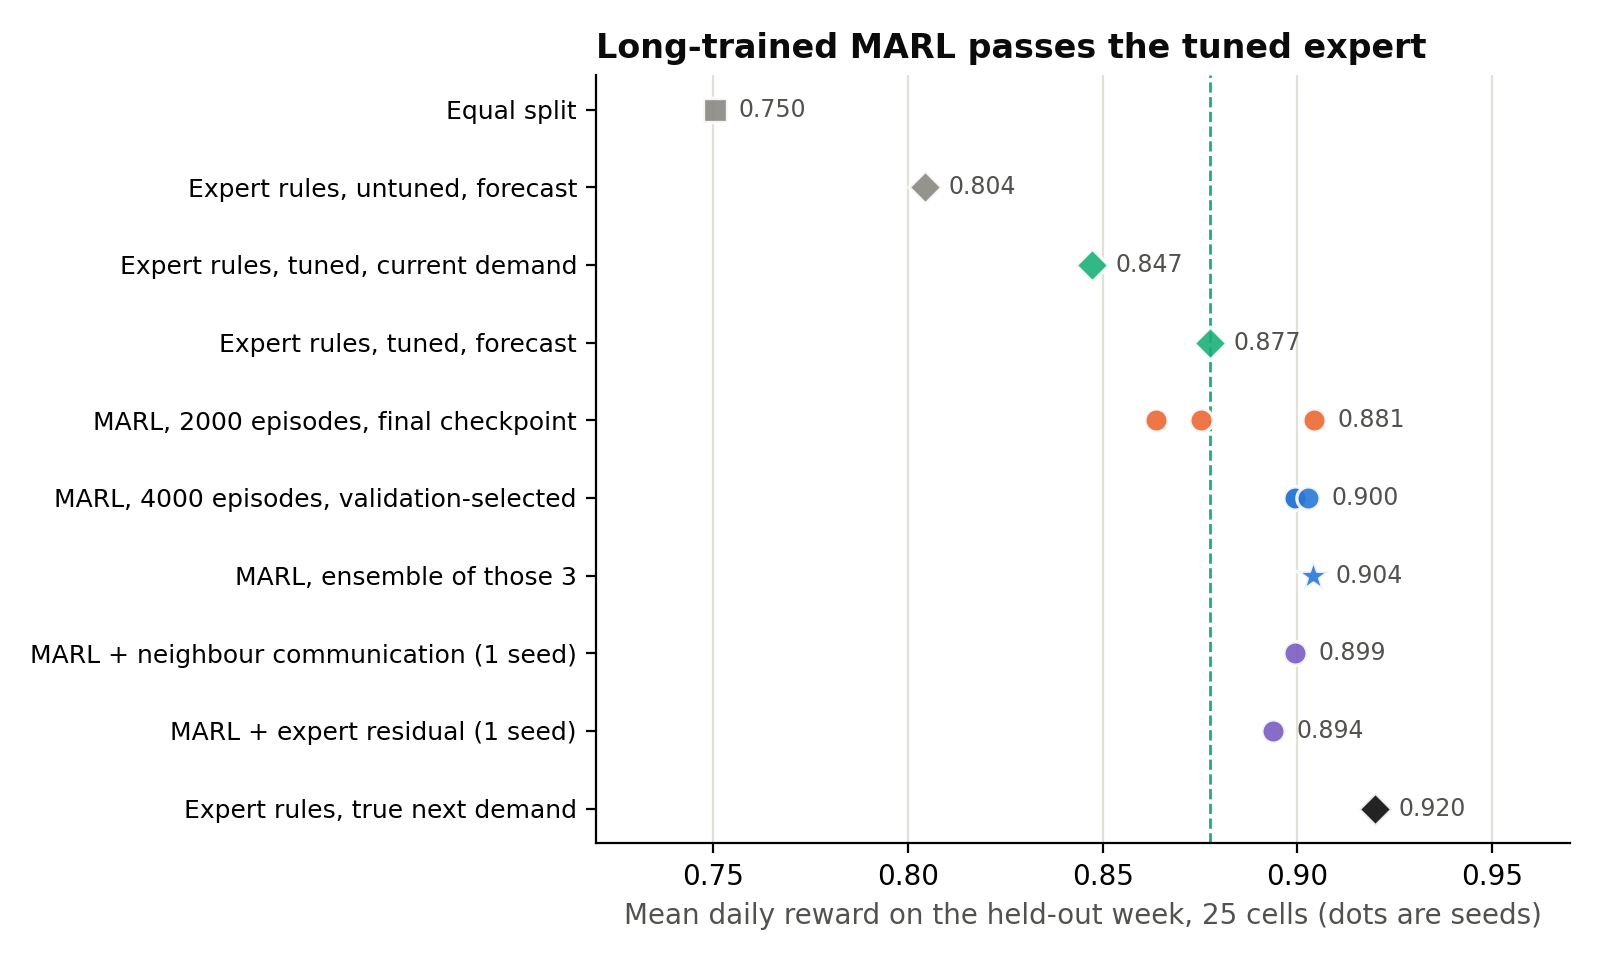
\includegraphics[width=0.9\textwidth,keepaspectratio]{unified_marl_best.png}
\caption{Long-protocol MARL against the tuned rules on the held-out week}
\label{fig:marl_best}
\end{figure}

Against the simple tuned rule, the learned controller is better on each of the seven test days at 9, 25 and 100 cells, by 0.023 to 0.024 in reward. Against the rich tuned rule the difference is about 0.005 or less, and at 25 and 100 cells the intervals include zero. So the off-policy controller matches a carefully tuned rule that knows the time of day and beats a simply tuned one, but it does not clearly beat the strongest hand-built rule. The on-policy learners of Section~\ref{sec:marl_ppo} do go beyond it. The 100-cell result rests on one seed, and its interval only describes the seven days.

\subsection{What the learned controller does}
Table~\ref{tab:marl_diagnosis} compares the allocations. The learned controller gives URLLC and mMTC about twice the capacity that the untuned rule gives them (shares of 0.23 and 0.09 against 0.11 and 0.04), so their SLAs are almost always met. It accepts a slightly lower share of eMBB demand served, and overall the reward is higher. This is a sensible policy and not an accident of the numbers, and the tuned rule ends up in the same place.

\begin{table}[htbp]
\centering
\caption{What the learned controller does differently (25 cells, held-out week; SLA rates, fraction of demand served, and mean capacity share per slice)}
\label{tab:marl_diagnosis}
\footnotesize
\begin{tabular}{|>{\centering\arraybackslash}p{\dimexpr 0.194\textwidth-2\tabcolsep\relax}|>{\centering\arraybackslash}p{\dimexpr 0.194\textwidth-2\tabcolsep\relax}|>{\centering\arraybackslash}p{\dimexpr 0.194\textwidth-2\tabcolsep\relax}|>{\centering\arraybackslash}p{\dimexpr 0.194\textwidth-2\tabcolsep\relax}|>{\centering\arraybackslash}p{\dimexpr 0.194\textwidth-2\tabcolsep\relax}|}
\hline
\textbf{Controller} & \textbf{SLA met (eMBB / URLLC / mMTC)} & \textbf{Demand served} & \textbf{Capacity share (eMBB / URLLC / mMTC)} & \textbf{Reward} \\ \hline
Shared MARL (2{,}000 episodes, seed 0) & 0.68 / 0.99 / 1.00 & 0.92 & 0.68 / 0.23 / 0.09 & 0.904 \\ \hline
Expert rule, forecast, untuned & 0.72 / 0.80 / 0.61 & 0.95 & 0.85 / 0.11 / 0.04 & 0.804 \\ \hline
Expert rule, true next demand & 0.72 / 1.00 / 1.00 & 0.95 & 0.85 / 0.11 / 0.04 & 0.920 \\ \hline
Equal split & 0.18 / 0.99 / 1.00 & 0.77 & 0.33 / 0.33 / 0.33 & 0.750 \\ \hline
\end{tabular}
\end{table}

\section{Training Variants}
\label{sec:marl_variants}
We tried several ways to improve the learner at 25 cells (Table~\ref{tab:marl_variants}): explicit communication between neighbouring actors, an expert-residual policy in which the actor outputs a correction to the allocation of the rule, a loss regularised towards the expert in the style of TD3+BC \cite{fujimoto2021minimalist}, and richer observations. None of them is clearly better than the plain shared actor trained with the long protocol and averaged. The on-policy learners of Section~\ref{sec:marl_ppo} are the exception. An actor with richer observations does not beat the rich tuned rule (a difference of $-0.007\pm0.009$, better on 2 of 7 days). The variants with one seed are only hints and should not be read as a ranking.

\begin{table}[htbp]
\centering
\caption{Training variants at 25 cells, held-out week reward}
\label{tab:marl_variants}
\footnotesize
\begin{tabular}{|>{\centering\arraybackslash}p{\dimexpr 0.300\textwidth-2\tabcolsep\relax}|>{\centering\arraybackslash}p{\dimexpr 0.170\textwidth-2\tabcolsep\relax}|>{\centering\arraybackslash}p{\dimexpr 0.170\textwidth-2\tabcolsep\relax}|}
\hline
\textbf{Variant} & \textbf{Seeds} & \textbf{Reward} \\ \hline
Shared DDPG, 2{,}000 episodes, with forecast & 3 & $0.881\pm0.021$ \\ \hline
Expert-regularised loss (TD3+BC style), no forecast & 3 & $0.844\pm0.065$ \\ \hline
Neighbour communication in the actor & 1 & 0.899 \\ \hline
Expert-residual policy & 1 & 0.894 \\ \hline
Communication and expert residual & 1 & 0.892 \\ \hline
Long protocol, ensemble of three actors & 3 & 0.904 \\ \hline
Long protocol with extra observations, ensemble & 2 & 0.892 \\ \hline
\end{tabular}
\end{table}

\section{On-Policy Baselines}
\label{sec:marl_ppo}
To compare with the off-policy design we also implemented independent PPO (IPPO) and a MAPPO-style variant \cite{schulman2017ppo, yu2022mappo, dewitt2020ippo}. The policy is a Gaussian over the four logits. Advantages come from generalised advantage estimation \cite{schulman2016gae} with $\lambda=0.95$ and $\gamma=0.9$ on the team reward, the clipping parameter is 0.2, and each update uses 10 episodes. In IPPO the actor and the value function of a cell only see that cell. In MAPPO the value function also sees the mean observation of the grid neighbours, which is the neighbourhood form of a centralised critic as in the DDPG critic, while the actor stays local. Both were trained for 8{,}000 episodes with the same checkpoint rule. Table~\ref{tab:marl_ppo} gives the outcome. All 12 runs end at almost the same reward, between 0.907 and 0.908, whichever variant or seed is used. This is higher than the off-policy controller of the previous sections (0.904) and higher than the rich tuned rule (0.899): averaged over the runs the difference to the rich rule is +0.009 $\pm$ 0.002, with a gain on 7 of 7 days, and every single run beats the rich rule on all seven days. The true-next-demand rule, which uses information no deployable controller has, is still higher at 0.920. IPPO and MAPPO give the same result, so in this environment the neighbourhood term in the value function brings no measurable benefit. The near-identical outcome of independent seeds suggests that the on-policy learner reliably finds the same good allocation behaviour, and that the remaining gap to the oracle comes from demand that cannot be predicted ten minutes ahead.

\begin{table}[htbp]
\centering
\caption{On-policy baselines at 25 cells (8{,}000 episodes, checkpoint chosen on validation days), held-out week}
\label{tab:marl_ppo}
\footnotesize
\begin{tabular}{|>{\centering\arraybackslash}p{\dimexpr 0.194\textwidth-2\tabcolsep\relax}|>{\centering\arraybackslash}p{\dimexpr 0.194\textwidth-2\tabcolsep\relax}|>{\centering\arraybackslash}p{\dimexpr 0.194\textwidth-2\tabcolsep\relax}|>{\centering\arraybackslash}p{\dimexpr 0.194\textwidth-2\tabcolsep\relax}|>{\centering\arraybackslash}p{\dimexpr 0.194\textwidth-2\tabcolsep\relax}|}
\hline
\textbf{Method} & \textbf{Seeds} & \textbf{Reward} & \textbf{Minus simple tuned expert} & \textbf{Minus rich tuned expert} \\ \hline
IPPO & 3 & $0.908\pm0.000$ & +0.030 & +0.009 \\ \hline
MAPPO & 9 & $0.908\pm0.000$ & +0.030 & +0.009 \\ \hline
Shared DDPG, long protocol, ensemble & 3 & 0.904 & +0.026 & +0.005 \\ \hline
\end{tabular}
\end{table}

\section{Robustness to Traffic Shifts}
\label{sec:marl_shift}
A controller trained on ordinary traffic may fail when the traffic changes. We therefore replayed the held-out week with the two scenario multipliers of Chapter~\ref{chap.8}, 6G growth and a massive-IoT surge. Table~\ref{tab:marl_shift} gives the results for controllers that were not retrained.

\begin{table}[htbp]
\centering
\caption{Controllers trained on ordinary traffic, run on shifted traffic (25 cells, held-out week, DDPG-MARL averaged over three 2{,}000-episode seeds)}
\label{tab:marl_shift}
\footnotesize
\begin{tabular}{|>{\centering\arraybackslash}p{\dimexpr 0.162\textwidth-2\tabcolsep\relax}|>{\centering\arraybackslash}p{\dimexpr 0.162\textwidth-2\tabcolsep\relax}|>{\centering\arraybackslash}p{\dimexpr 0.162\textwidth-2\tabcolsep\relax}|>{\centering\arraybackslash}p{\dimexpr 0.162\textwidth-2\tabcolsep\relax}|>{\centering\arraybackslash}p{\dimexpr 0.162\textwidth-2\tabcolsep\relax}|>{\centering\arraybackslash}p{\dimexpr 0.162\textwidth-2\tabcolsep\relax}|}
\hline
\textbf{Traffic} & \textbf{Equal split} & \textbf{Expert tuned on ordinary} & \textbf{Expert re-tuned on this traffic} & \textbf{MARL with forecast} & \textbf{MARL without forecast} \\ \hline
Ordinary traffic & 0.750 & 0.877 & 0.877 & 0.881 & 0.851 \\ \hline
6G growth (eMBB $\times$1.3, URLLC $\times$2, mMTC $\times$3) & 0.615 & 0.762 & 0.762 & 0.724 & 0.692 \\ \hline
Massive IoT (mMTC $\times$10) & 0.666 & 0.725 & 0.735 & 0.672 & 0.685 \\ \hline
\end{tabular}
\end{table}

When the traffic shifts, the learned controllers lose a lot of reward, and a rule that is re-tuned on the new traffic is clearly better. The forecast input helps the learned policy on ordinary traffic and under 6G growth (by about 0.03) and costs about 0.01 under the surge, so its effect is not consistent. Training on a mixture of scenarios solves the problem (Table~\ref{tab:marl_robust}). The policy trained on the mixture beats an expert re-tuned on the training days of each scenario in every traffic condition on average. The gain is clear on ordinary traffic and under 6G growth, and it is within noise under the massive-IoT surge.

\begin{table}[htbp]
\centering
\caption{MARL trained on a mixture of traffic scenarios (two seeds, actors averaged), against an expert rule re-tuned on each scenario's own training days}
\label{tab:marl_robust}
\footnotesize
\begin{tabular}{|>{\centering\arraybackslash}p{\dimexpr 0.300\textwidth-2\tabcolsep\relax}|>{\centering\arraybackslash}p{\dimexpr 0.170\textwidth-2\tabcolsep\relax}|>{\centering\arraybackslash}p{\dimexpr 0.170\textwidth-2\tabcolsep\relax}|>{\centering\arraybackslash}p{\dimexpr 0.170\textwidth-2\tabcolsep\relax}|}
\hline
\textbf{Test traffic} & \textbf{MARL reward} & \textbf{Difference (95\% CI)} & \textbf{Days better} \\ \hline
Ordinary traffic & 0.904 & +0.026 $\pm$ 0.003 & 7/7 \\ \hline
6G growth & 0.780 & +0.018 $\pm$ 0.002 & 7/7 \\ \hline
Massive IoT & 0.738 & +0.003 $\pm$ 0.003 & 6/7 \\ \hline
\end{tabular}
\end{table}

\section{Earlier B5G MADDPG Development}
\label{sec:b5g-maddpg}
Before the unified Milan environment existed, we implemented MADDPG on the B5G network-slicing release. The environment loads the graph, routing and slice data and makes one observation for every node that starts at least one flow. The policy is a shared actor with a critic that looks at the local state and allocation. The first comparisons used equal allocation, a rule-based heuristic and an untrained actor.

While developing it we found that the slice identifiers restart for each slice type. Using the identifier alone as the agent key therefore mixed up the records of eMBB, URLLC and mMTC and made the statistics invalid, so we excluded the affected results. The B5G release also has no usable latency and packet-loss fields, which an SLA-based reward needs. These experiments show that the replay, training and evaluation pipeline runs, but they do not show that the learned policy improves real QoS.

\section{Chapter Conclusion}
\label{sec:marl-conclusion}
Three things came out of this chapter. First, a parameter-shared actor with a neighbourhood critic keeps its size and its reward when the network grows from 9 to 100 cells, while a central agent does not. Second, with a fair training budget, checkpoints chosen on validation days and averaged seeds, the learned controller beats a simply tuned expert rule on every test day at 9, 25 and 100 cells. Third, the off-policy controller only matches a richer rule that is tuned for each time of day, but the PPO-family learners, trained for 8{,}000 episodes, beat that rule on every test day in every run at 25 cells. Learned controllers also need retraining, or training on a mixture of scenarios, when traffic changes a lot. Whether the forecast helps the learned controller is discussed in Chapter~\ref{chap.8}.

\chapter{Integrated Evaluation and the Digital Twin}
\label{chap.8}
\section{Introduction}
This chapter evaluates the whole pipeline in the unified environment of Chapter~\ref{chap.4}. We ask whether knowing the demand of the next interval helps allocation, whether the forecast helps the learned controller, how the controllers behave over the whole city, and what a Digital Twin adds to the work. We then describe the Digital Twin dataset and its what-if scenarios, and finish by testing the surrogate environment against a packet-level simulator.

\section{Value of the Forecast}
\label{sec:forecast-value}
On the held-out week the retrained forecaster of Chapter~\ref{chap.6} has a mean squared error that is 18\%, 33\% and 31\% lower than persistence for eMBB, URLLC and mMTC. To see what this is worth for allocation, we ran the same expert rule with three kinds of knowledge about the next ten minutes: the current demand, the TGNN forecast, and the true next demand, which is an upper bound for any forecast. Table~\ref{tab:forecast-value} gives the result.

\begin{table}[htbp]
\centering
\caption{Reward of the expert rule with different knowledge of the next ten minutes, held-out week (default targets)}
\label{tab:forecast-value}
\footnotesize
\begin{tabular}{|>{\centering\arraybackslash}p{\dimexpr 0.121\textwidth-2\tabcolsep\relax}|>{\centering\arraybackslash}p{\dimexpr 0.121\textwidth-2\tabcolsep\relax}|>{\centering\arraybackslash}p{\dimexpr 0.121\textwidth-2\tabcolsep\relax}|>{\centering\arraybackslash}p{\dimexpr 0.121\textwidth-2\tabcolsep\relax}|>{\centering\arraybackslash}p{\dimexpr 0.121\textwidth-2\tabcolsep\relax}|>{\centering\arraybackslash}p{\dimexpr 0.121\textwidth-2\tabcolsep\relax}|>{\centering\arraybackslash}p{\dimexpr 0.121\textwidth-2\tabcolsep\relax}|>{\centering\arraybackslash}p{\dimexpr 0.121\textwidth-2\tabcolsep\relax}|}
\hline
\textbf{Cells} & \textbf{Equal split} & \textbf{Current demand} & \textbf{TGNN forecast} & \textbf{True next demand} & \textbf{Forecast minus current (95\% CI)} & \textbf{Days better} & \textbf{Gap recovered} \\ \hline
9 & 0.785 & 0.794 & 0.825 & 0.945 & +0.030 $\pm$ 0.008 & 7/7 & 20\% \\ \hline
25 & 0.750 & 0.775 & 0.804 & 0.920 & +0.029 $\pm$ 0.006 & 7/7 & 20\% \\ \hline
49 & 0.728 & 0.758 & 0.788 & 0.902 & +0.029 $\pm$ 0.004 & 7/7 & 20\% \\ \hline
100 & 0.735 & 0.765 & 0.794 & 0.908 & +0.029 $\pm$ 0.004 & 7/7 & 20\% \\ \hline
\end{tabular}
\end{table}

\begin{figure}[htbp]
\centering
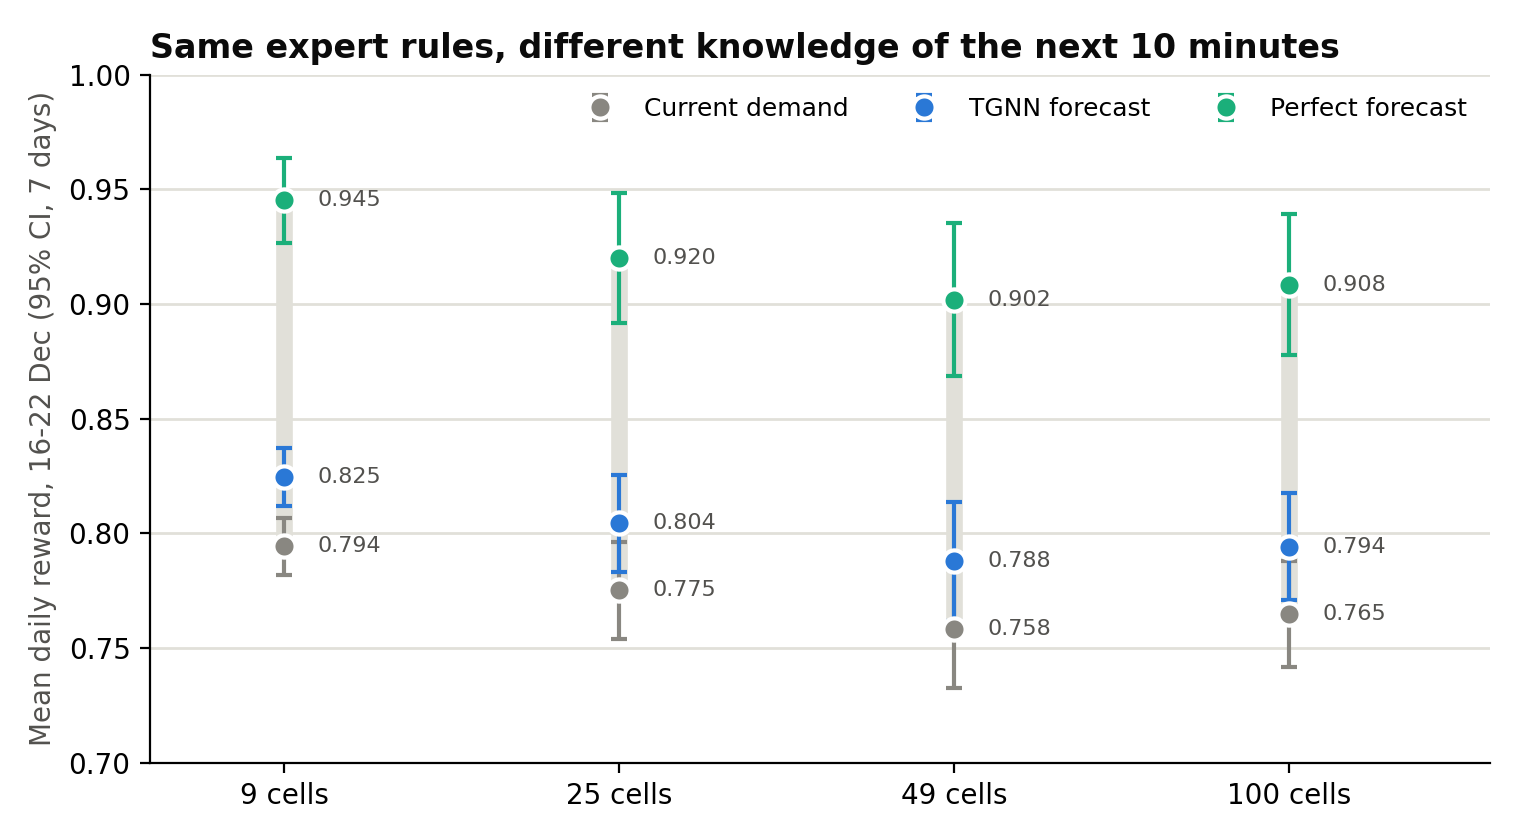
\includegraphics[width=0.85\textwidth,keepaspectratio]{unified_prediction_value.png}
\caption{Value of prediction for the expert rule at four network sizes}
\label{fig:forecast-value}
\end{figure}

The forecast improves the expert rule by about 0.03 in reward at every network size and on all seven test days, with intervals of about 0.004 to 0.008. It closes about one fifth of the gap to perfect knowledge. An earlier estimate of 0.05 came from two test days and a forecaster trained on five days. With 39 training days and a whole week of testing, the benefit is smaller but better established. Using the value of the previous day at the same time as a forecast does not work: its mean reward is 0.74 to 0.78 at every size, which is below that of current demand.

\section{The Forecast and the Learned Controller}
\label{sec:forecast-marl}
We also gave the forecast to the MARL controller as an extra input. Table~\ref{tab:forecast-marl} shows that at this training budget, with three seeds, it made no reliable difference. Giving the controller the true next-interval demand did not help either.

\begin{table}[htbp]
\centering
\caption{MARL with and without forecast input (25 cells, three seeds, mean $\pm$ sample standard deviation)}
\label{tab:forecast-marl}
\footnotesize
\begin{tabular}{|>{\centering\arraybackslash}p{\dimexpr 0.300\textwidth-2\tabcolsep\relax}|>{\centering\arraybackslash}p{\dimexpr 0.170\textwidth-2\tabcolsep\relax}|}
\hline
\textbf{Input to the MARL controller} & \textbf{Held-out reward} \\ \hline
No forecast & $0.778\pm0.048$ \\ \hline
Forecast from the first (5-day) TGNN & $0.765\pm0.051$ \\ \hline
Forecast from the retrained TGNN & $0.772\pm0.073$ \\ \hline
True next-interval demand & $0.762\pm0.057$ \\ \hline
\end{tabular}
\end{table}

\begin{figure}[htbp]
\centering
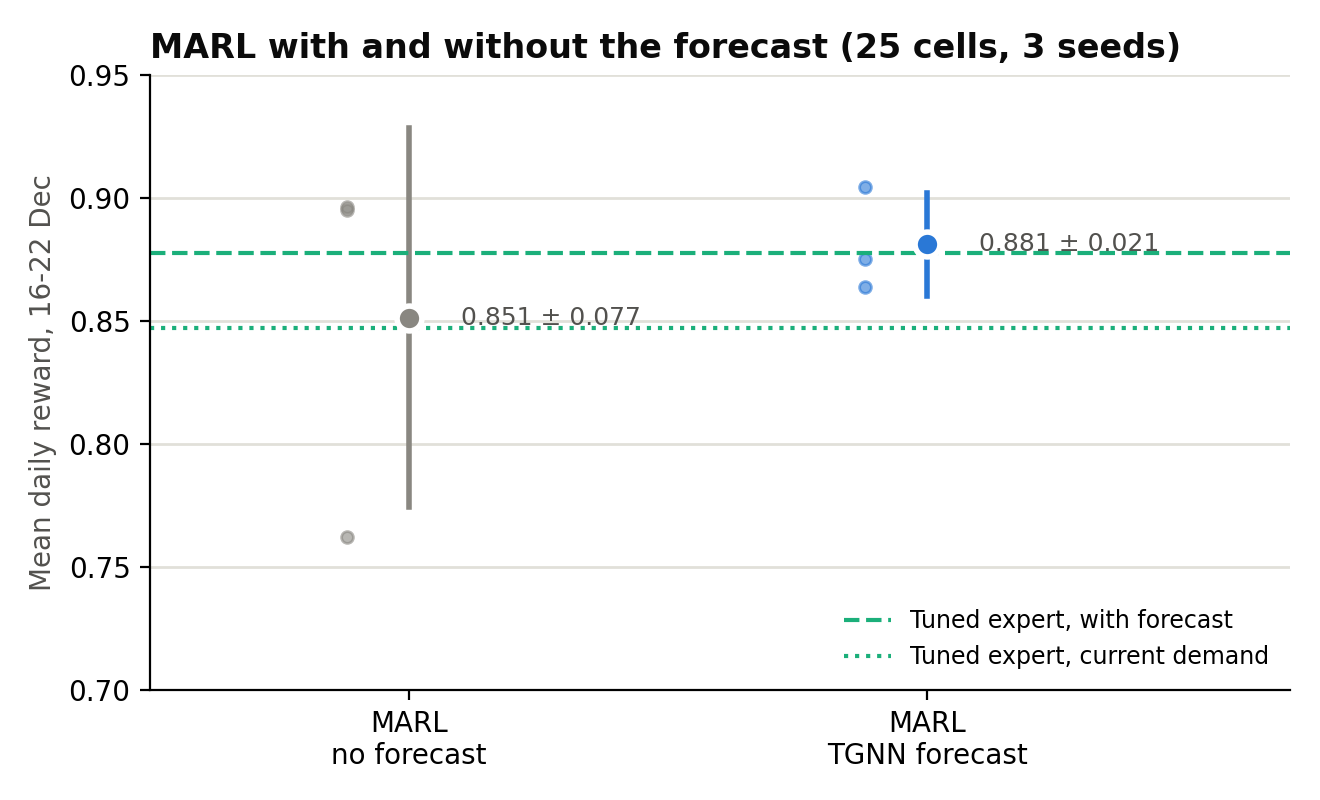
\includegraphics[width=0.8\textwidth,keepaspectratio]{unified_forecast_ablation.png}
\caption{Learned controller with and without the forecast}
\label{fig:forecast_for_marl}
\end{figure}

The three rewards differ by less than their sample standard deviations of 0.05 to 0.06, so the experiment shows neither a clear gain nor a clear loss. Under shifted traffic the effect on the learned policy even changes sign (Section~\ref{sec:marl_shift}). We therefore claim that forecasting helps the rule-based controller, and we have not shown that it helps the learned one. The forecast is still useful: the Digital Twin gate of Section~\ref{sec:gate} uses it to predict the outcome of a proposed allocation.

\section{Controllers Across the Whole City}
\label{sec:city-controllers}
We ran the three controllers of the Slice Twin monitor (Chapter~\ref{chap.9}) on all 10{,}000 Milan cells for one day, Wednesday 6 November 2013, with scripted incidents. Static divides the capacity equally. Reactive applies the expert rule to the current demand. Predictive applies it to the city-wide forecast. The forecaster was not trained on this day.

\begin{table}[htbp]
\centering
\caption{Controllers on all 10{,}000 cells, Wednesday 6 November 2013 (reward of the whole city, the dense block and the outer city)}
\label{tab:city-controllers}
\footnotesize
\begin{tabular}{|>{\centering\arraybackslash}p{\dimexpr 0.194\textwidth-2\tabcolsep\relax}|>{\centering\arraybackslash}p{\dimexpr 0.194\textwidth-2\tabcolsep\relax}|>{\centering\arraybackslash}p{\dimexpr 0.194\textwidth-2\tabcolsep\relax}|>{\centering\arraybackslash}p{\dimexpr 0.194\textwidth-2\tabcolsep\relax}|>{\centering\arraybackslash}p{\dimexpr 0.194\textwidth-2\tabcolsep\relax}|}
\hline
\textbf{Controller} & \textbf{SLA met (eMBB / URLLC / mMTC)} & \textbf{Whole city} & \textbf{Dense block} & \textbf{Outer city} \\ \hline
Static & 0.919 / 0.997 / 1.000 & 0.974 & 0.709 & 0.977 \\ \hline
Reactive & 0.975 / 0.711 / 0.568 & 0.839 & 0.735 & 0.840 \\ \hline
Predictive & 0.975 / 0.786 / 0.601 & 0.868 & 0.773 & 0.869 \\ \hline
\end{tabular}
\end{table}

In the dense block the Predictive controller scores highest (0.773 against 0.735 and 0.709), as in Section~\ref{sec:forecast-value}. Over the whole city, however, Static scores highest (0.974 against 0.868 and 0.839). Most cells are lightly loaded, and when URLLC and mMTC traffic is close to zero the rule gives those slices very little capacity, so they miss their targets when traffic comes back. The outer city has most of the cells, and this outweighs the benefit of forecasting. An earlier run reported 0.935 for the Predictive controller over the city. That came from over-allocation caused by a bias of the block-trained forecaster in the outer cells, and the table above replaces it. Since this is a single day, it shows how the controllers behave and does not rank them.

\section{The Digital Twin Dataset}
\label{sec:dt-dataset}
No public dataset contains topology, per-slice traffic, QoS metrics, SLA outcomes and allocation decisions together, so we generated one from the unified environment (\texttt{src/\allowbreak unified/\allowbreak twin\_\allowbreak dataset.py}). Each row is one cell in one 10-minute interval. The data is stored as Parquet files on the project drive, and summaries and samples are in the repository. We made two builds (Table~\ref{tab:dt-size}), with 393.6 million rows in total.

\begin{table}[htbp]
	\centering
	\caption{Size of the Digital Twin dataset}
	\label{tab:dt-size}
	\small
	\resizebox{\textwidth}{!}{%
	\begin{tabular}{|l|c|c|c|r|c|}
		\hline
		\textbf{Build} & \textbf{Cells} & \textbf{Days} & \textbf{Scenarios} & \textbf{Rows} & \textbf{Size} \\
		\hline
		Core year (central $20\times 20$ block) & 400 & 364 & 6 & 125{,}796{,}000 & 30.8 GB \\
		Full city (whole grid) & 10{,}000 & 62 & 3 & 267{,}810{,}000 & 40.5 GB \\
		\hline
		\textbf{Total} & & & & \textbf{393{,}606{,}000} & \\
		\hline
	\end{tabular}}
\end{table}

\paragraph{Provenance.}
The 62 recorded days are real Telecom Italia Milan data \cite{barlacchi2015}. The other days of the core year are bootstrapped from real days of the same weekday, with 20\% growth per year and a little random variation. The columns \texttt{source} and \texttt{source\_date} say whether a row is real or bootstrapped. Latency and jitter follow curves calibrated on the 6G RAN telemetry. The radio fields follow the 3GPP CQI table \cite{3gpp38214} and the power follows the EARTH base-station model \cite{auer2011}. The slice mapping, the industrial zones, the per-user rates and the packet sizes are our own assumptions.

\paragraph{Structure.}
Each row has 122 columns. Twenty are for identity and calendar, 3 for control, 8 for events and state, 11 for radio and capacity, 6 for the neighbourhood and 3 for energy. There are 63 per-slice fields (21 for each slice, including the demand 10, 30 and 60 minutes ahead as forecasting targets), 2 for the reward and 6 for noisy telemetry. Appendix~\ref{app:columns} lists all of them.

\paragraph{Validation.}
We ran all six scenarios for three days before the full build and checked five things. All scenarios have the same interval and cell rows. Traffic is conserved under energy saving, since the traffic that sleeping cells hand over equals what the neighbours receive. The industrial and massive-IoT multipliers are applied exactly. 1.0\% of the telemetry is missing, as designed. The 10- and 60-minute targets equal the demand of the same cell one and six rows later. These are automated tests in the repository. They show that the generator is consistent with itself, not that it agrees with a packet-level simulator.

\section{What-if Scenarios}
\label{sec:scenarios}
All scenarios share the same days, the same behaviour policy and the same random noise, so any difference between two scenarios comes from the scenario. Table~\ref{tab:scenarios} gives the results for the core year.
\begin{table}[htbp]
	\centering
	\caption{Scenarios of the core year}
	\label{tab:scenarios}
	\footnotesize
	\begin{tabular}{|p{2.3cm}|p{4.6cm}|p{3.4cm}|p{1.3cm}|p{1.8cm}|}
		\hline
		\textbf{Scenario} & \textbf{What changes} & \textbf{SLA met (eMBB / URLLC / mMTC)} & \textbf{Reward} & \textbf{Energy (MWh)} \\
		\hline
		baseline & Recorded traffic, no incidents & 0.704 / 0.731 / 0.651 & 0.763 & 3{,}473 \\
		\hline
		events & Adds flash crowds, outages, interference, URLLC bursts, mMTC storms, capacity degradation & 0.703 / 0.730 / 0.651 & 0.763 & 3{,}473 \\
		\hline
		growth\_6g & eMBB $\times$1.3, URLLC $\times$2, mMTC $\times$3 & 0.553 / 0.696 / 0.610 & 0.688 & 3{,}648 \\
		\hline
		energy\_saving & Quiet cells sleep 01:00--05:00 and hand traffic to neighbours & 0.703 / 0.737 / 0.659 & 0.766 & 3{,}435 \\
		\hline
		industrial\_urllc & Industrial cells: URLLC $\times$4 in weekday shifts & 0.693 / 0.723 / 0.646 & 0.756 & 3{,}481 \\
		\hline
		massive\_iot & mMTC $\times$10, a further $\times$3 at the start of each hour & 0.554 / 0.710 / 0.524 & 0.660 & 3{,}628 \\
		\hline
	\end{tabular}
\end{table}

The scaled-traffic scenarios behave as intended. growth\_6g lowers the eMBB compliance from 0.704 to 0.553, and massive\_iot lowers the mMTC compliance from 0.651 to 0.524 and uses the most energy. The events scenario is almost the same as the baseline because over 99.8\% of its rows have no event. The effect only shows when the rows are grouped by event type (Table~\ref{tab:events}).

\begin{table}[htbp]
	\centering
	\caption{Effect of each injected event (core year, events scenario)}
	\label{tab:events}
	\small
	\begin{tabular}{|l|r|c|c|}
		\hline
		\textbf{Event} & \textbf{Rows} & \textbf{SLA met (eMBB / URLLC / mMTC)} & \textbf{Reward} \\
		\hline
		none & 20{,}932{,}659 & 0.704 / 0.730 / 0.651 & 0.763 \\
		flash crowd & 19{,}740 & 0.217 / 0.683 / 0.598 & 0.532 \\
		cell outage & 985 & 0.000 / 0.095 / 0.019 & 0.019 \\
		interference spike & 8{,}883 & 0.577 / 0.697 / 0.629 & 0.704 \\
		URLLC burst & 814 & 0.608 / 0.510 / 0.575 & 0.631 \\
		mMTC storm & 1{,}966 & 0.658 / 0.730 / 0.344 & 0.679 \\
		capacity degradation & 953 & 0.323 / 0.710 / 0.647 & 0.578 \\
		\hline
	\end{tabular}
\end{table}

\paragraph{Energy saving across the city.} We also ran the energy-saving scenario on the whole city for 62 days (Table~\ref{tab:energy}). When lightly loaded cells sleep from 01:00 to 05:00, night-time energy drops by 19.6\%, from 1{,}983 MWh to 1{,}593 MWh, and total energy over the period drops by 3.2\%. The price is that the URLLC compliance of the awake cells falls from 0.761 to 0.720, because their mean load rises from 0.045 to 0.066. The saving has to be read together with this loss of QoS.

\begin{table}[htbp]
	\centering
	\caption{Night-time sleep across the city (01:00 to 05:00, 62 days)}
	\label{tab:energy}
	\small
	\begin{tabular}{|l|c|c|}
		\hline
		\textbf{Measure} & \textbf{Baseline} & \textbf{Energy saving} \\
		\hline
		Night-time energy (MWh) & 1983 & 1593 (19.6\% lower) \\
		Night cell-intervals asleep & 0\% & 47.6\% \\
		SLA met, awake cells (eMBB / URLLC / mMTC) & 0.983 / 0.761 / 0.724 & 0.976 / 0.720 / 0.693 \\
		Mean load of awake cells & 0.045 & 0.066 \\
		\hline
	\end{tabular}
\end{table}

\section{The Digital Twin as an Approval Gate}
\label{sec:gate}
A Digital Twin is only useful if it can check a decision before the decision is applied, and the unified environment now has a gate that does this. Before a cell's allocation is applied, the twin predicts the outcome of the next interval for the proposed allocation and for a safe fallback. It uses the QoS model of the environment and the TGNN forecast of the demand in that interval. The fallback is the expert rule tuned on the training days. The proposal is approved if its predicted reward is at least that of the fallback, and otherwise the fallback is applied. The gate works cell by cell.

We measured the gate on the held-out week with controllers whose proposals are sometimes bad, as when a learning agent explores online. These were the trained MARL actor with Gaussian noise of standard deviation $\sigma$ added to its logits, and an equal split. Table~\ref{tab:gate} gives the reward with and without the gate.

\begin{table}[htbp]
\centering
\caption{Effect of the approval gate on the held-out week (25 cells, mean over the three MARL seeds)}
\label{tab:gate}
\footnotesize
\begin{tabular}{|>{\centering\arraybackslash}p{\dimexpr 0.300\textwidth-2\tabcolsep\relax}|>{\centering\arraybackslash}p{\dimexpr 0.170\textwidth-2\tabcolsep\relax}|>{\centering\arraybackslash}p{\dimexpr 0.170\textwidth-2\tabcolsep\relax}|>{\centering\arraybackslash}p{\dimexpr 0.170\textwidth-2\tabcolsep\relax}|}
\hline
\textbf{Controller} & \textbf{Reward without gate} & \textbf{Reward with gate} & \textbf{Proposals approved} \\ \hline
MARL, logit noise $\sigma= 0$ & 0.900 & 0.898 & 72\% \\ \hline
MARL, logit noise $\sigma= 0.5$ & 0.805 & 0.876 & 7\% \\ \hline
MARL, logit noise $\sigma= 1.0$ & 0.707 & 0.877 & 3\% \\ \hline
MARL, logit noise $\sigma= 2.0$ & 0.574 & 0.877 & 1\% \\ \hline
Equal split & 0.750 & 0.879 & 2\% \\ \hline
\end{tabular}
\end{table}

The gate has two sides. For a good controller ($\sigma=0$) it gives nothing: the reward is the same to within 0.003, and the gate still rejects about a quarter to a third of the proposals. For degraded controllers it recovers almost everything that was lost and brings each case back to the reward of the fallback alone (0.8775). So the gate is a safety measure and not an improvement. It stops the result from dropping below the fallback when a proposal is poor, and how well it works depends on how good the twin's prediction is. Our twin uses the same QoS model as the environment it is tested in, so this experiment cannot tell us how accurate the gate would be on a real network.

\section{Checking the Surrogate Against a Packet-Level Simulator}
\label{sec:simu5g}
The QoS model of our environment is a calibrated surrogate. To test it against a packet-level simulator we ran a load sweep in Simu5G 1.7.0 (OMNeT++ 6.4, INET 4.7), with one gNodeB and ten UEs receiving downlink UDP traffic in messages of 1000 bytes. The offered load went from 11\% to 125\% of the measured capacity of 56.1 Mbps, with three repetitions per point. Table~\ref{tab:simu5g_sweep} and Figure~\ref{fig:simu5g_sweep} show the delay.

\begin{table}[htbp]
\centering
\caption{Simu5G load sweep (10 UEs, one gNodeB, downlink capacity 56.1 Mbps, 1000-byte messages, 6 s, mean of three repetitions)}
\label{tab:simu5g_sweep}
\footnotesize
\begin{tabular}{|>{\centering\arraybackslash}p{\dimexpr 0.300\textwidth-2\tabcolsep\relax}|>{\centering\arraybackslash}p{\dimexpr 0.170\textwidth-2\tabcolsep\relax}|>{\centering\arraybackslash}p{\dimexpr 0.170\textwidth-2\tabcolsep\relax}|>{\centering\arraybackslash}p{\dimexpr 0.170\textwidth-2\tabcolsep\relax}|}
\hline
\textbf{Utilisation} & \textbf{Median delay (ms)} & \textbf{95th-percentile delay (ms)} & \textbf{Received (Mbps)} \\ \hline
0.11 & 4.5 & 5.0 & 6.0 \\ \hline
0.21 & 4.5 & 4.9 & 12.0 \\ \hline
0.36 & 4.4 & 5.0 & 20.0 \\ \hline
0.54 & 4.5 & 5.0 & 30.0 \\ \hline
0.68 & 4.7 & 6.9 & 38.0 \\ \hline
0.78 & 4.6 & 6.8 & 44.0 \\ \hline
0.86 & 6.0 & 6.8 & 48.0 \\ \hline
0.93 & 6.1 & 434.5 & 50.5 \\ \hline
1.00 & 5.9 & 1376.2 & 50.1 \\ \hline
1.07 & 5.8 & 780.8 & 50.7 \\ \hline
1.25 & 11.1 & 211.9 & 55.6 \\ \hline
\end{tabular}
\end{table}

\begin{figure}[htbp]
\centering
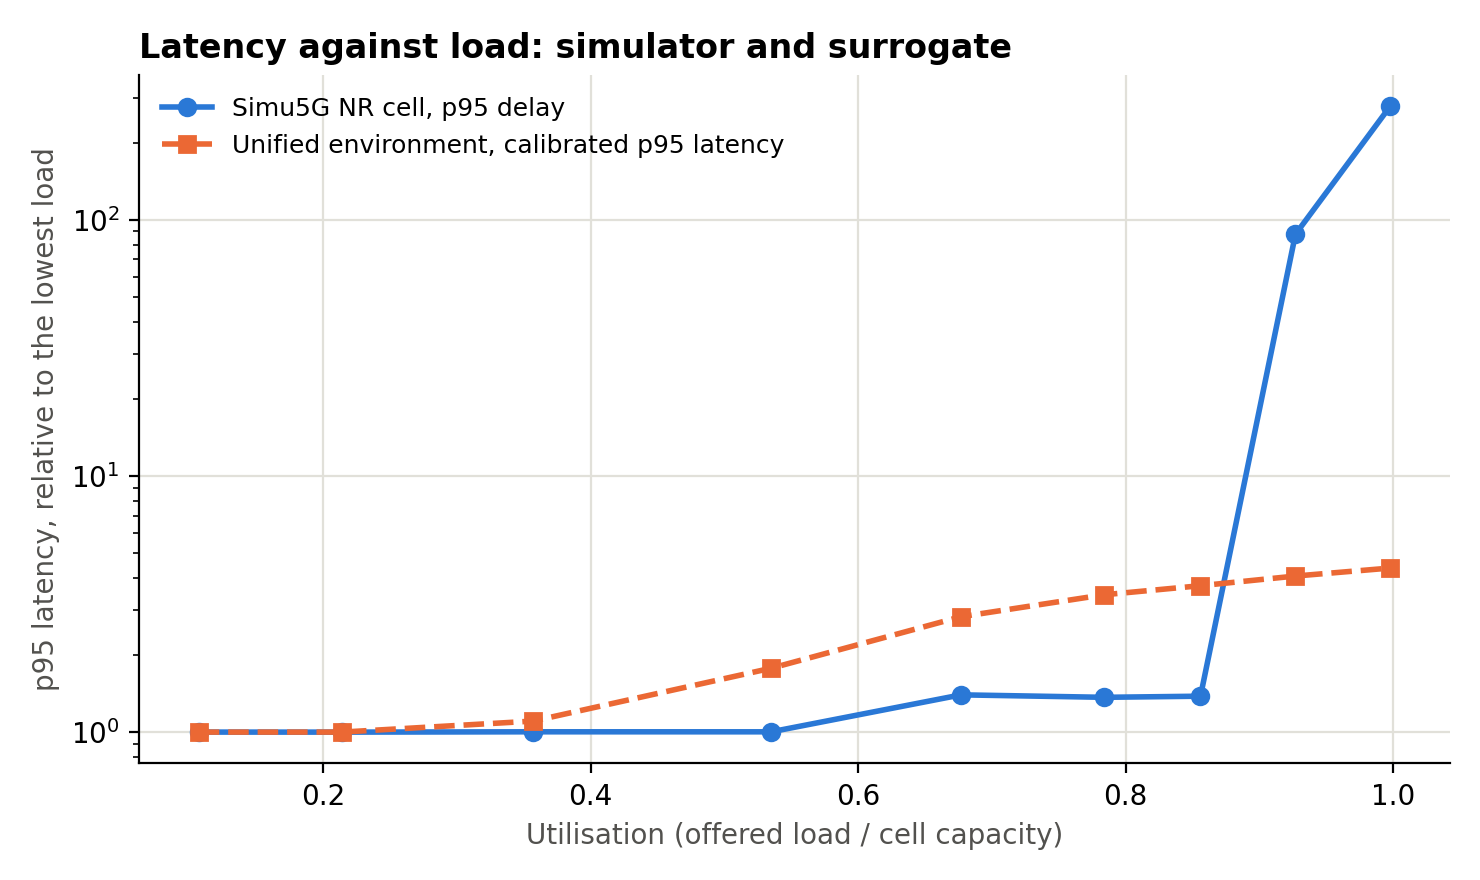
\includegraphics[width=0.8\textwidth,keepaspectratio]{simu5g_latency_vs_load.png}
\caption{Delay against load: Simu5G and the surrogate of the environment (normalised)}
\label{fig:simu5g_sweep}
\end{figure}

The two models agree on the ordering: the rank correlation of the normalised 95th-percentile delay between Simu5G and our surrogate is 0.93. They do not agree on the shape. In Simu5G the delay stays flat at about 5 ms until the load reaches about 93\% of capacity, and then it jumps, to 434 ms at 93\% and above one second at full load. Our surrogate rises slowly from 53\%, and the load at which its 95th-percentile delay doubles is 68\% rather than 93\%. The surrogate is therefore more cautious than the simulator at moderate load and far too optimistic beyond saturation. The 5 ms floor in the sweep comes from the scheduling of the simulator. We read this as a check of shape and ranking, not as a calibration of absolute values.

Because the controllers were developed on the surrogate, we repeated the evaluation on a latency curve with the shape of the Simu5G sweep (flat, then a cliff at capacity). Table~\ref{tab:simu5g_eval} gives the result. The ranking of the methods is the same as on the default curve: the forecast-fed rule beats the current-demand rule, and the learned controllers, which were not retrained, score about 0.95, above the rule tuned on this curve (0.942) and close to the rule that is given the true next demand (0.957). MAPPO retrained on this curve (three seeds) reaches 0.969, above that rule as well. The ordering of the controllers therefore does not depend on the smooth shape of the surrogate.

\begin{table}[htbp]
\centering
\caption{Controllers on the Simu5G-shaped latency curve (25 cells, held-out week)}
\label{tab:simu5g_eval}
\footnotesize
\begin{tabular}{|>{\centering\arraybackslash}p{\dimexpr 0.300\textwidth-2\tabcolsep\relax}|>{\centering\arraybackslash}p{\dimexpr 0.170\textwidth-2\tabcolsep\relax}|>{\centering\arraybackslash}p{\dimexpr 0.170\textwidth-2\tabcolsep\relax}|}
\hline
\textbf{Controller} & \textbf{Runs} & \textbf{Reward} \\ \hline
Equal split & 1 & 0.814 \\ \hline
Expert rule, untuned, current & 1 & 0.909 \\ \hline
Expert rule, tuned under this curve, current & 1 & 0.913 \\ \hline
Expert rule, untuned, forecast & 1 & 0.940 \\ \hline
Expert rule, tuned under this curve, forecast & 1 & 0.942 \\ \hline
Expert rule on the true next demand, untuned & 1 & 0.957 \\ \hline
IPPO, trained on the default curve, not retrained & 3 & $0.953\pm0.002$ \\ \hline
MAPPO, trained on the default curve, not retrained & 9 & $0.953\pm0.001$ \\ \hline
MAPPO, retrained under this curve & 3 & $0.968\pm0.000$ \\ \hline
DDPG-MARL, trained on the default curve, not retrained & 3 & $0.948\pm0.003$ \\ \hline
\end{tabular}
\end{table}

\section{The Role of the Digital Twin in This Work}
\label{sec:dt-role}
The Digital Twin has three roles in this work.
\begin{itemize}
    \item \textbf{Training and evaluation.} The unified environment combines real Milan traffic with modelled slice demand, allocation actions, QoS estimates, SLA outcomes and rewards.
    \item \textbf{Scenario generation.} The 393.6-million-row dataset, six what-if scenarios and automated consistency checks allow controlled evaluation under different conditions.
    \item \textbf{Approval gate.} Section~\ref{sec:gate} shows that the twin can reject poor proposals before they are applied, which protects the result from a degraded controller.
\end{itemize}
The main limit is that the QoS comes from a calibrated surrogate whose reference telemetry is itself simulated. The fall of the mean gap from 0.086 to 0.021 shows a good fit, not an independent validation, and the Simu5G sweep shows that the shape of the surrogate differs from a packet-level model. The twin therefore supports comparisons between controllers under assumptions that we state; it has not been validated for deployment decisions.

\section{Summary}
In the unified environment the TGNN forecast improves the expert rule by about 0.03 in reward at every network size and on all seven test days, which closes about one fifth of the gap to perfect knowledge. We have not shown that it improves the learned controller. Over the whole city the static split scores highest, because the rule starves the quiet slices, while in the dense block the predictive controller is best. The Digital Twin dataset supports six scenarios, among them an energy-saving policy that cuts night-time energy by 19.6\% at a URLLC cost on the awake cells. The twin also works as an approval gate that protects the result from poor proposals, and a Simu5G sweep shows that the surrogate agrees with the simulator on the order of delays but not on the shape of the delay curve.

\chapter{Prototype: Slice Twin Monitor}
\label{chap.9}
\section{Introduction}
The prototype is \emph{Slice Twin}, a monitor that runs in the browser and shows how different controllers split the bandwidth of each cell between eMBB, URLLC and mMTC over one day of real Milan traffic. It makes the environment of Chapter~\ref{chap.4} and the experiments of Chapters~\ref{chap.7} and~\ref{chap.8} something you can click through. The source is in \texttt{app/slice\_twin} of the project repository, and the monitor, a results dashboard and a project brief are published at \texttt{https://fyp-a09.github.io/6G/}.

\section{Purpose and Design}
Slice Twin lets you watch what the controllers do, see how incidents hit each slice, and compare forecast-based allocation with simpler allocation on the same data.

\paragraph{Data shown.}
One held-out day is replayed: Wednesday 6 November 2013, which the forecaster was not trained on (days 5 and 6 are excluded from its training for this reason). The traffic is real Telecom Italia Milan data \cite{barlacchi2015}. We inject scripted incidents so that the controllers have something to react to: an mMTC storm, an interference spike, a cell outage, a backhaul degradation, a flash crowd and a URLLC burst on the central block. The city view adds four more, namely a firmware push in the north-west, wide-area interference in the east, storm damage in the south and a crowd at San Siro. Every incident is labelled and described in the interface. They are scripted for the demonstration and are not real events.

\paragraph{Interaction model.}
The interface is modelled on Cisco Packet Tracer. In Realtime mode the day plays continuously at a speed you choose. In Simulation mode the playback stops at each new event. An event list gives the time, cells and description of every incident, and a timeline marks the incidents and lets you jump to any time of the day.

\section{Views and Controllers}
\label{sec:slice-views}
\paragraph{Block view.} The 100 central cells ($10\times10$) are drawn as rings. The segments of a ring show how the cell splits its capacity between the three slices, and moving packets show the traffic that is served. Selecting a cell opens an inspector with its demand, its allocation, its latency against the target and the SLA status of each slice.

\paragraph{City view.} All 10{,}000 cells are drawn as a map that can be coloured by real traffic, by load or by SLA misses, with landmarks (Duomo, Milano Centrale, San Siro, Linate airport, Navigli, Citt\`a Studi) and the active incidents. Selecting a cell compares the three controllers on it over the day, and a cell of the central block can be opened in the block view. City-wide curves show the bandwidth given to each slice and the fraction of cells meeting each SLA, with an option to show the gain over the Reactive controller.

\paragraph{Controllers.} Three controllers run in the same environment (Chapter~\ref{chap.4}).
\begin{itemize}
	\item \textbf{Static:} an equal split of each cell's capacity that never changes.
	\item \textbf{Reactive:} the expert rule, which gives URLLC and mMTC enough capacity to stay under their SLA-safe utilisation and the rest to eMBB, using the current demand.
	\item \textbf{Predictive:} the same rule fed with the TGNN forecast of the next ten minutes (the city-trained forecaster of Chapter~\ref{chap.6} in the city view).
\end{itemize}
These are the controllers of Section~\ref{sec:city-controllers}, so the monitor agrees with Table~\ref{tab:city-controllers}. On the central block (Table~\ref{tab:block-controllers}) the Predictive controller is better than Reactive, and an oracle that knows the true next demand would be better still. Over the whole city the Static split scores highest.

\begin{table}[htbp]
\centering
\caption{Controllers on the 100 central cells, Wednesday 6 November 2013}
\label{tab:block-controllers}
\footnotesize
\begin{tabular}{|>{\centering\arraybackslash}p{\dimexpr 0.300\textwidth-2\tabcolsep\relax}|>{\centering\arraybackslash}p{\dimexpr 0.170\textwidth-2\tabcolsep\relax}|>{\centering\arraybackslash}p{\dimexpr 0.170\textwidth-2\tabcolsep\relax}|}
\hline
\textbf{Controller} & \textbf{SLA met (eMBB / URLLC / mMTC)} & \textbf{Reward} \\ \hline
Static & 0.13 / 0.98 / 1.00 & 0.709 \\ \hline
Reactive & 0.59 / 0.74 / 0.57 & 0.735 \\ \hline
Predictive & 0.59 / 0.82 / 0.61 & 0.768 \\ \hline
Oracle (true next demand) & 0.59 / 1.00 / 1.00 & 0.876 \\ \hline
\end{tabular}
\end{table}

\section{Technical Notes}
\label{sec:slice-tech}
\paragraph{Technology and data flow.}
Slice Twin is a static web application with no code on a server. All the calculations are done beforehand, and the browser (HTML, CSS and JavaScript) only reads the prepared files and draws the views (Figure~\ref{fig:slice-flow}).
\begin{figure}[htbp]
	\centering
	\small
	\fbox{\parbox{0.92\textwidth}{\centering
	Milan traffic $\rightarrow$ unified environment $\rightarrow$ three controllers with incidents and forecast (Python, offline)\\
	$\downarrow$\\
	\texttt{data.json} (block), \texttt{city.json} and \texttt{city.bin.gz} (city)\\
	$\downarrow$\\
	Browser reads the files and draws the views and charts}}
	\caption{Data flow of the Slice Twin monitor}
	\label{fig:slice-flow}
\end{figure}
The files are produced by \texttt{showcase.py} for the block view and \texttt{showcase\_city.py} for the city view, both in \texttt{src/unified}. The city data is stored compactly. For each interval and cell, one byte holds the log-scaled demand. For each controller, one byte holds the load (scaled by 250) and one byte holds flags: bits 0 to 2 say whether each slice meets its SLA, bit 3 marks an event and bit 4 an outage. The compressed binary file is a few megabytes, so the browser can handle 10{,}000 cells over 144 intervals and three controllers.

\paragraph{How to run it.}
From the root of the repository, \texttt{python -m http.server 8765 --directory app/slice\_twin} starts the monitor at \texttt{http://localhost:8765}. To regenerate the data, run \texttt{showcase.py}, then \texttt{forecast\_\allowbreak city\_\allowbreak v2.py} once to train the city forecaster, and then \texttt{showcase\_\allowbreak city.py}; the Milan files must be on the project drive. A GitHub Actions workflow publishes the monitor, the results dashboard and the project brief to GitHub Pages whenever the site or monitor folders change.

\paragraph{Demonstration.}
Figure~\ref{fig:slice-city} shows the city view at 17:30 on the demonstration day. In the top image the cells are coloured by real traffic, with the storm-damage incident in the south marked, and in the bottom image by SLA misses under the Reactive controller.
\begin{figure}[htbp]
    \centering
    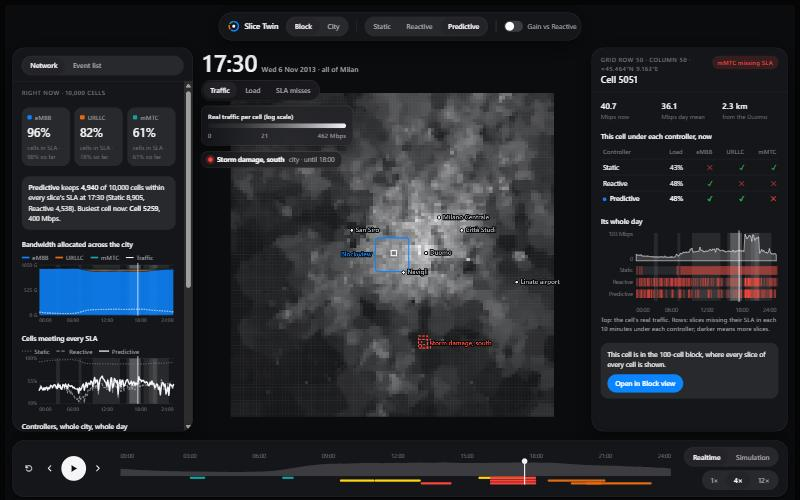
\includegraphics[width=0.92\textwidth]{slice_twin_city_dark.jpg}\\[1.2em]
    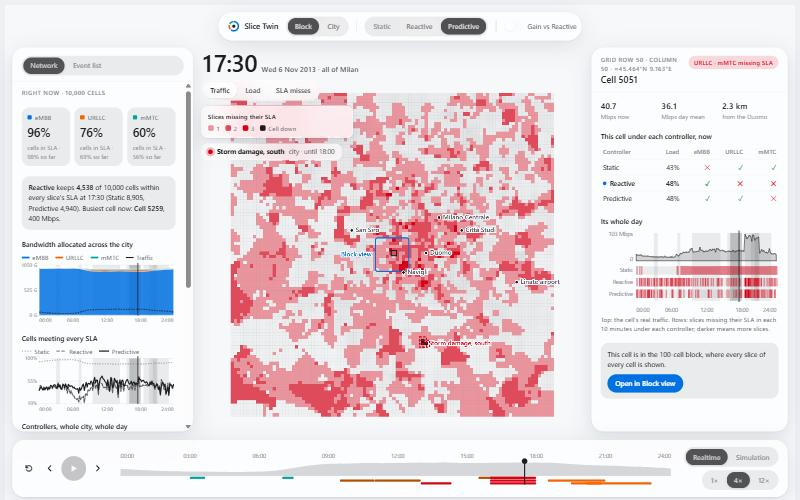
\includegraphics[width=0.92\textwidth]{slice_twin_city_light.jpg}
    \caption{City view at 17:30: cells coloured by real traffic (top, dark theme) and by SLA misses under the Reactive controller (bottom, light theme).}
    \label{fig:slice-city}
\end{figure}

\section{Contribution to the Project}
\label{sec:slice-contrib}
The Slice Twin monitor is the working product of the project, and the code, the unified environment and the dataset in the repository stand behind it. It also works as a demonstration. A viewer can see that the predictive controller helps in the dense centre, that the static split holds up better on quiet outer cells, and how each incident affects each slice. Its limits are the limits of its data: it shows one held-out day with scripted incidents, and it does not control a live or simulated network. It is a tool for monitoring and comparison, not a deployed controller.

\chapter{Conclusion and Scope for further Research}
\label{chap.10}
\section{Summary}
\label{Summary}
This thesis asked whether a 6G slicing controller allocates bandwidth better when it knows the demand of the next interval, and whether decentralised multi-agent reinforcement learning suits the task better than a single central agent. We built a pipeline of self-supervised learning, a temporal graph neural network and multi-agent reinforcement learning, and tested it in a unified slicing environment built on real Telecom Italia Milan traffic. All results come from a held-out week, with checkpoints and rule targets chosen on separate validation days.

\paragraph{Does knowing the next interval help?}
For the rule-based controller, yes, by a modest amount. Replacing the current demand by the TGNN forecast raises the reward by about 0.03 at every size from 9 to 100 cells, on all seven test days, and recovers about one fifth of the gap to perfect knowledge (Chapter~\ref{chap.8}). The forecaster itself beats persistence on all 10{,}000 cells, with mean squared error lower by 18\%, 33\% and 31\% for eMBB, URLLC and mMTC. For the learned controller the answer is not established: giving it the forecast changed its reward by less than the seed-to-seed variation.

\paragraph{Is multi-agent learning better than a single central agent?}
Yes, in two ways. A parameter-shared actor of 19{,}332 parameters works from 9 to 100 cells, while the central agent needs 114{,}468 to 604{,}048 parameters and its reward falls from about 0.43 to 0.27 (Chapter~\ref{chap.7}). With a long training budget, checkpoints chosen on validation days and seeds averaged, the learned controller also beats a simply tuned expert rule on every test day at 9, 25 and 100 cells, by 0.023 to 0.026 in reward. The off-policy controller does not clearly beat a richer rule that is tuned for each time of day and cell class: its difference to that rule is between +0.001 and +0.005 and its interval includes zero at 25 and 100 cells. The on-policy learners (IPPO and MAPPO, 12 runs) do beat that rule: their mean reward is 0.908 against 0.899, a gain of 0.009 $\pm$ 0.002 on 7 of 7 days at 25 cells, and every run is better on all seven days. They do not reach the rule that is given the true next demand (0.920).

\section{Contributions}
\label{Contributions}
\begin{enumerate}
    \item \textbf{A unified slicing environment.} Since no public dataset joins topology, per-slice traffic, quality of service, SLA outcomes and allocation actions, we built an environment from real Milan traffic and grid data, with latency calibrated on public 6G RAN telemetry and load-coupled interference. Each component is marked as real, calibrated or modelled.
    \item \textbf{A fair evaluation protocol for MARL.} Train, validation and test periods are separate, baselines are tuned on the training days, results are paired by day with intervals, and the strongest rule is part of the comparison.
    \item \textbf{A measurement of what prediction is worth.} The value of the forecast is stated as the reward gained and as the fraction of the gap to perfect knowledge, at four network sizes.
    \item \textbf{A city-scale forecasting finding.} A forecaster trained on the dense centre failed in the periphery, with error 10.8 times that of persistence, because it had learned the traffic level of the centre. Per-cell scaling, patch training and more training days removed the failure.
    \item \textbf{A clean negative result for SSL.} Pretraining did not beat strong raw-feature baselines on de-duplicated 5G-NIDD flows at any label budget.
    \item \textbf{A Digital Twin that checks decisions.} The approval gate recovers the reward lost to poor proposals, and a Simu5G sweep tests the surrogate against a packet-level simulator.
    \item \textbf{A dataset and a prototype.} The dataset has 393.6 million rows and 122 columns, six what-if scenarios and injected incidents, and the Slice Twin monitor provides a visual interface to the results.
\end{enumerate}
The work also documents corrections that changed early results: a label-ordered split and duplicate flows in 5G-NIDD, a slice-indexing error in the B5G environment, a city-wide forecast bias, and an earlier estimate of the value of the forecast that was reduced from 0.05 to 0.03 once the test period was extended to a week.

\section{Limitations}
\label{sec:limitations}
\paragraph{Statistical strength.}
The test is one week (seven days, which are not independent) in one city, with at most three seeds per learned controller and one seed at 100 cells. The intervals reported describe the variation across those days, not across weeks, cities or training runs. A stronger study would use ten or more seeds and more weeks.

\paragraph{Comparison with the best hand-built rule.}
The off-policy learned controller only matches a rule tuned per time of day and cell class; the PPO-family learners beat it by about 0.009 reward, a small margin, and were tested only at 25 cells with the default QoS curve. The case for learning also rests on removing the manual tuning and on its behaviour as the network grows. The central-agent baseline is also weak: its reward fell during training, so the result shows that this central design performs poorly, not that every centralised design would.

\paragraph{Fidelity of the surrogate model.}
QoS comes from a calibrated surrogate, and the telemetry used for calibration is itself simulated. The latency spread was fitted on the same SLA-against-load curve that is used for evaluation, so the drop in the mean gap from 0.086 to 0.021 measures fit and is not independent validation. The Simu5G sweep agrees with the surrogate on the order of delays but not on their shape: the packet-level delay is flat until about 93\% of capacity and then rises steeply, whereas the surrogate rises gradually from about half of capacity. The slice mapping, demand scale, interference coupling and reward weights are modelling assumptions.

\paragraph{Negative results.}
Self-supervised pretraining did not outperform raw features for 5G-NIDD classification or for the Milan forecast, so the contribution of the SSL stage to the pipeline is not demonstrated. The forecast has not been shown to help the learned controller. Over the whole city the static split beats the predictive controller because the rule starves quiet slices, and the city comparison covers a single day. The forecaster was trained once, without an ablation of its parts and without graph-free or published spatio-temporal baselines.

\paragraph{The Digital Twin claim.}
The twin trains controllers, evaluates them, generates scenarios and gates proposals. The gate uses the same QoS model as the environment in which it is tested, so how well it would predict outcomes on a real network is not shown. The controllers have not been validated against a live or packet-level network. The prototype is a monitor of one held-out day with scripted incidents.

\section{Future Work}
\label{sec:future-work}
\paragraph{Stronger statistics and baselines.}
Repeat the experiments with ten or more seeds and several test weeks, add the 100-cell runs with more seeds, and add a graph-free forecaster and published spatio-temporal models together with an ablation of the city forecaster.

\paragraph{Closing the simulator gap.}
Connect the project's own 19-gNodeB scenario to Simu5G, run controllers in closed loop with it and record latency, jitter and loss, which would also supply the latency and loss data that the B5G dataset lacks. Calibrate the surrogate on the measured delay curve, in particular the flat-then-cliff shape.

\paragraph{SSL with richer inputs.}
Test SSL on inputs where hand-crafted features are not available, such as raw radio measurements or longer sequences, and with an encoder that uses neighbouring cells and earlier intervals.

\paragraph{Forecast-aware learning.}
Investigate why the forecast does not help the learned controller, for example with a longer training budget, a design in which the forecast is part of the critic, or training on forecast errors.

\paragraph{Semantic slicing and O-RAN traces.}
Extend the reward with semantic criteria suggested by the literature, and check the surrogate against public O-RAN and testbed traces that contain measured PRB use, throughput and channel quality.

\paragraph{Deployment.}
Move the monitor and controllers from replay towards a closed loop with a simulator or testbed, and study decision latency inside the control interval, coordination between neighbouring cells and the cost of reconfiguration.

\section{Concluding Remarks}
Within these limits, the work shows three things. Predicting traffic before allocating bandwidth helps a rule-based controller. A parameter-shared multi-agent controller scales to larger networks where a central one does not, and it beats rules whose targets were tuned on the training days. And a forecaster has to be trained on the whole city if it is going to be used there. Two questions stay open: whether a learned controller can make real use of the forecast, and whether a packet-level simulator agrees with our surrogate beyond the ordering of delays.

\appendix
\chapter{Dataset Columns and Experimental Settings}
\label{app:columns}
\section{Columns of the Digital Twin Dataset}
Each row of the dataset is one cell in one 10-minute interval and has 122 columns. 59 are general columns and 21 are repeated for each of the three slices with the prefix \texttt{eMBB\_}, \texttt{URLLC\_} or \texttt{mMTC\_}, giving 63. The general columns are:

\begin{center}
\footnotesize
\begin{tabular}{lll}
\texttt{scenario} & \texttt{policy} & \texttt{modulation} \\
\texttt{interval} & \texttt{idle\_share} & \texttt{spectral\_efficiency\_bps\_hz} \\
\texttt{day\_index} & \texttt{event\_type\_code} & \texttt{power\_w} \\
\texttt{date} & \texttt{event\_type} & \texttt{energy\_wh} \\
\texttt{interval\_of\_day} & \texttt{event\_id} & \texttt{energy\_efficiency\_mbit\_per\_j} \\
\texttt{hour} & \texttt{anomaly} & \texttt{rehomed\_in\_mbps} \\
\texttt{minute} & \texttt{cell\_asleep} & \texttt{rehomed\_out\_mbps} \\
\texttt{weekday} & \texttt{capacity\_factor} & \texttt{handover\_users\_est} \\
\texttt{month} & \texttt{interference\_factor} & \texttt{reconfiguration\_churn} \\
\texttt{day\_of\_year} & \texttt{capacity\_mbps} & \texttt{anomaly\_score} \\
\texttt{iso\_week} & \texttt{spare\_capacity\_mbps} & \texttt{all\_slices\_sla\_ok} \\
\texttt{season} & \texttt{total\_demand\_mbps} & \texttt{reward} \\
\texttt{is\_weekend} & \texttt{total\_served\_mbps} & \texttt{team\_reward} \\
\texttt{is\_holiday} & \texttt{prbs\_used} & \texttt{obs\_total\_demand\_mbps} \\
\texttt{is\_business\_hours} & \texttt{load} & \texttt{obs\_embb\_latency\_p95\_ms} \\
\texttt{is\_night} & \texttt{neighbour\_load} & \texttt{obs\_load} \\
\texttt{source} & \texttt{neighbour\_mean\_demand\_mbps} & \texttt{obs\_sinr\_db} \\
\texttt{source\_date} & \texttt{neighbour\_all\_sla\_ok} & \texttt{obs\_cqi} \\
\texttt{cell\_id} & \texttt{sinr\_db} & \texttt{telemetry\_missing} \\
\texttt{zone} & \texttt{cqi} &  \\
\end{tabular}
\end{center}

The per-slice columns (to be prefixed with the slice name) are:

\begin{center}
\footnotesize
\begin{tabular}{lll}
\texttt{demand\_mbps} & \texttt{share} & \texttt{queue\_kbit} \\
\texttt{demand\_next\_10min\_mbps} & \texttt{prbs} & \texttt{latency\_p50\_ms} \\
\texttt{demand\_next\_30min\_mbps} & \texttt{allocated\_mbps} & \texttt{latency\_p95\_ms} \\
\texttt{demand\_next\_60min\_mbps} & \texttt{utilisation} & \texttt{jitter\_ms} \\
\texttt{demand\_1h\_mean\_mbps} & \texttt{served\_mbps} & \texttt{loss} \\
\texttt{demand\_delta\_mbps} & \texttt{throughput\_per\_user\_mbps} & \texttt{sla\_margin\_ms} \\
\texttt{users\_est} & \texttt{packets} & \texttt{sla\_ok} \\
\end{tabular}
\end{center}

\section{Experimental Settings}
\label{app:status}
\begin{itemize}
	\item \textbf{Data split.} Training days 1 to 40; validation days 41 to 44; test days 45 to 51 (16--22 December 2013). Days 5 and 6 are excluded from forecaster training.
	\item \textbf{Environment.} 10-minute intervals, 144 per day, capacity 100 Mbps per cell, interference coupling 0.3, reward $0.7\,S+0.3\,F-0.1\,H$, headroom targets $(0.65,0.5,0.65)$ by default.
	\item \textbf{Forecaster.} Two GraphSAGE layers and a GRU cell with 64 hidden units, residual output head, window of six intervals, $32\times32$ patches, per-cell 95th-percentile scaling, trained on 39 days with the epoch chosen on days 41 to 44.
	\item \textbf{MARL.} Shared actor of 19{,}332 parameters, neighbourhood critic, discount 0.9, $\tau=0.01$, learning rates $3\times10^{-4}$ and $10^{-3}$, replay 50{,}000; long protocol 4{,}000 episodes with validation every 250 episodes, seeds 0 to 2.
	\item \textbf{PPO family.} 8{,}000 episodes, ten episodes per update, clip 0.2, four epochs, entropy bonus 0.003, GAE with $\lambda=0.95$.
	\item \textbf{Code and results.} Everything is in the repository \texttt{FYP-A09/6G}: environment and learners in \texttt{src/unified}, result files in \texttt{reports/unified}, figures in \texttt{docs/figures}, tests in \texttt{tests/test\_unified.py}.
\end{itemize}


%\addcontentsline{toc}{chapter}{\textbf{References}}
\newpage
\renewcommand{\bibname}{References}
\bibliographystyle{ieeetr}
\addcontentsline{toc}{chapter}{References}
\bibliography{mybib}

\chapter*{List of Publications \\ \large(Based on the Research Work)}
\addcontentsline{toc}{chapter}{List of Publications Based on the Research Work}
\textbf{\Large Papers Published}\\
None so far.\vspace{0.4cm}

\noindent \textbf{\Large Papers Communicated}\\
None so far.

\clearpage
\chapter*{Planned Publications}
\addcontentsline{toc}{chapter}{Planned Publications}
\noindent\textbf{\Large Survey Paper (in preparation)}
\begin{enumerate}
	\item \textbf{Title:} Digital Twin-Assisted Network Slicing for 6G Using Self-Supervised Learning, Temporal Graph Neural Networks and Multi-Agent Reinforcement Learning: A Survey
	\item \textbf{Journal:} IEEE Communications Surveys \& Tutorials (tentative)
\end{enumerate}
\vspace{0.6cm}

\noindent\textbf{\Large Technical Paper (in preparation)}
\begin{enumerate}
	\item \textbf{Title:} Forecast-Informed Multi-Agent Control of 6G Network Slices in a City-Scale Digital Twin
	\item \textbf{Journal:} IEEE Transactions on Network and Service Management (tentative)
\end{enumerate}

\end{document}
	
	